%!TeX root=../tese.tex
%("dica" para o editor de texto: este arquivo é parte de um documento maior)
% para saber mais: https://tex.stackexchange.com/q/78101/183146

% Os capítulos de compõem a dissertação/tese, com numeração normal, podem
% ser inseridos diretamente aqui ou "puxados" de outros arquivos.
% Em alguns (raros) casos, pode ser interessante usar \include ao
% invés de \input: https://tex.stackexchange.com/a/32058/183146
%!TeX root=../tese.tex
%("dica" para o editor de texto: este arquivo é parte de um documento maior)
% para saber mais: https://tex.stackexchange.com/q/78101/183146

%% ------------------------------------------------------------------------- %%
\chapter{Introduction}
\label{cap:introduction}

Social networks have all but taken over contemporary daily life. From the
eponymous socializing, to reading news, to expressing ourselves, social media
has creeped into every corner of society. Most of its side-effects, it could be
argued, are positive (shortening distances, political accountability, social
organizing), but they are not perfect institutions.

Social media companies already face significant backlash for their questionable
business model and ethics. Cambridge Analytica's election meddling, Facebook's
subliminal experiments, YouTube's problem with disturbing content marketed at
kids, and Twitter's bot infestation are just a few recent scandals that have put
the societal role of social media into question.

One particular controversy that has taken over public discourse around social
networks is the role that their algorithms might have in radicalizing users,
specially younger ones. The aforementioned experiments conducted by Facebook to
influence people's emotions and the proliferation of more than questionable
videos aimed at children on YouTube are instances that seem to corroborate the
notion that there is something fundamentally wrong with these companies'
algorithms.

News organizations, in general, have been skeptical of social networks.
Journalists and specialists alike argue that social media's algorithms
(specially recommender algorithms) are tuned to peddle conspiracy theories,
extremist views, and false information. This would be the source cause for a
plethora of what they consider contemporary evils: religious extremism,
anti-democratic leaders, widespread depression among teenagers, anti-science
movements, etc.

This narrative, of course, has been questioned for a variety of reasons. Some
say that it is self serving: traditional news organizations are being displaced
by social media and it would be convenient for them to mine the public's trust
in them. Others claim that these recommender algorithms are not to blame for
political polarization and that social networks even have a tendency to favor
more left-wing viewpoints.

The debate around the role of recommender systems in social media radicalization
is still, unfortunately, too recent and based in anecdotes. Since its impacts
are all but universal, more quality research is vital to inform both the public
and opinion makers about if and how much recommendation algorithms influence
social media users.

This dissertation aims to further such research. The rest of Chapter 1 is
dedicated to core concepts covered in the rest of the work, ending in subsection
1.4, which tackles the main hypothesis of this dissertation. Chapter 2 contains
the literature review, Chapter 3 explains the experiments already conducted and
their results, and Chapter 4 is about next steps.

\section{Social Networks}
\label{sec:social_networks}

Social networking services, also referred to as social networks and social
media, are notoriously difficult to define. Some definitions might be too narrow
(excluding instant messaging services), while some might be too broad (including
technologies such as telephone networks). Most definitions include some common
features:

\begin{itemize}
  \item Internet-based
  \item Focus on user-generated content
  \item Users have profiles
  \item Users can connect
\end{itemize}

While social-networking-like applications already existed in Usenet, Geocities,
launched in 1994, is usually regarded as the first major social network.
Friendster and Myspace followed in 2003, with Orkut and Facebook slightly
lagging behind in 2004. Each hit their peak at different moments and different
countries, but Facebook overtook all of them in 2009 when it became the most
popular social networking service in the world, still maintaining the title over
11 years latter at the moment of writing.

Even though all aforementioned social networks are multimedia, that is, users
can post text, photos and videos, some of the most popular services focus on a
specific type of media. For instance, YouTube (2009) centers around videos,
WhatsApp (2009) and WeChat (2011) were originally designed for text-based
communication, and Instagram's (2010) main focus is photos.

Some social media services, very much in agreement with McLuhan's teachings,
have what could be considered a ``style''. Instagram's content, for example,
tends toward more personal (i.e. egoic) photos and videos. As of November 28th,
2020, six of the top 20 most-liked posts on Instagram are from american
socialite Kylie Jenner, consisting of four photos of her daughter and two of her
ex-boyfriend. Even though there are many different niches inside Instagram,
personal posts seam to have an edge over other kinds of content.

Twitter, unlike most other social networks, allows for asymmetrical connections,
meaning users can follow profiles without being followed back. This enables the
emergence of Twitter communities (e.g. Fintwit, Black Twitter) that can be
largely self referential and/or organized around certain subjects. Facebook
users, on the other hand, can belong to groups, user-moderated profiles that
might revolve around any particular topics of interest; there are groups that
organize pet owners and groups that organize neonazis.

Parallel to all other features and idiosyncrasies, there lay the recommendation
algorithms. While a few social networking services (e.g. WhatsApp) do not
recommend any content or profiles to the user, most do and, according to recent
studies, these recommendations have become the main drivers of interactions.

\section{Recommender Systems}
\label{sec:recommender_systems}

Recommender systems (sometimes called recommendation systems or recomender
algorithms) first appeared in 1992 under the name ``collaborative filtering'',
even though that term nowadays refers to a subclass of recommender systems. The
aim of such an algorithm is providing users with personalized product or service
recommendations, an essential task when considering the ever increasing number
of possible videos to watch, music to listen, products to buy.

The input of a recommender system is usually information about the preferences
(ratings, likes/dislikes, watch time, etc.) of consumers for a set of items.
Preference information can be gathered from explicit behaviors (e.g. rating a
product in a scale ranging from 0 to 5 stars) or from implicit behaviors (e.g.
how much time the user lingers on a product's page). These data can be combined
with information about the user (age, political leaning, etc.) in order to
create the best possible representation of the user's preferences.

The output of these systems can come in the form of a prediction or a list of
recommended items. In the first case, the goal of the algorithm is approximating
the rating a user would attribute to a yet unrated item, while the second type
of output involves gathering the items that most likely would interest the user.
Simple recommender systems that suggest items similar to the one being queried
do not necessarily involve rating predictions, but it is common to have the list
of rcommended items based on the ratings the algorithms estimated the user would
give to those items.

Most recommender systems follow into one of four categories according to the
filtering algorithm they use, that it, the strategy for generating predictions
or selecting the top-N items: content-based filtering, demographic filtering,
collaborative filtering, and hybrid filtering.

Content-based filtering leverages characteristics of the content in order to
generate the recommendations. One such algorithm might use the genres of watched
movies in order to recommend new ones, while another might analyse the sound
signature of a song to recommend similar ones, but, either way, all
content-based systems establish a similarity between items as a basis for
recommendations. Analogously, demographic filtering uses demographic data to
establish a similarity between users and recommend items positively rated by
similar people.

Collaborative filtering algorithms also recommend items that similar users
liked, but, in this case, the similarity between users is based on past ratings
and not demographic information. Hybrid filtering usually mix collaborative
methods with either content-based or demographic filtering.

As with other knowledge-based systems, recommendation algorithms have quickly
incorporated neural networks and other machine learning techniques over the past
few years. Even though the implementation of YouTube's recommendation algorithm
is a trade secret, it is known to gather enormous amounts of data about the
user's interaction with the website and to require Google's own TPUs in order to
be trained. It also involves two distinct steps: candidate generation (when the
billions of videos available on the platform are quickly narrowed down to a few
hundreds that might be relevant) and ranking (when the algorithm actually
attempts to predict the score a user would implicitly give to the candidate
videos).

Another relevant aspect of recommender systems that is well-exemplified by
YouTube is the use of balancing factors such as novelty, dispersity, and
stability. In the case of Google's video giant, there is a baked-in bias for
recency, strongly favoring newer videos in detriment of older content.

\section{Radicalization}
\label{sec:radicalization}

Opinion polarization is far from a recent phenomenon, and social media is only
the most recent communication medium where it can be detected and studied. An
important question is whether it facilitates or attenuates polarization:
anecdotal evidence might suggest that social network structures incentivize
users to gather into antagonistic communities, but this could be a result of
people simply being more likely to express their preferences online, not of some
intrinsic property of social media.

One possible byproduct of polarization is radicalization. Despite not being
entirely different phenomena, these concepts deserve distinct levels of
attention. While polarization can be considered a natural part of democratic
discourse, radicalization only happens when certain conditions are met. UNESCO
defines radicalization as:

\begin{itemize}
  \item The individual person's search for fundamental meaning, origin and
        return to a root ideology;
  \item The individual as part of a group's adoption of a violent form of
        expansion of root ideologies and related oppositionist objectives;
  \item The polarization of the social space and the collective construction of
        a threatened ideal 'us' against 'them,' where the others are dehumanized
        by a process of scapegoating.
\end{itemize}

The third point is of special importance to the distinction between polarization
and radicalization. The first might be a simple consequence of democratic
disagreements between opposing parties, but the latter involves a dehumanization
of the opposition, which can lead to extremism: radicalism so intense that the
only effective strategy is physically exterminating the opposition.

Understanding how polarization might lead to radicalization (and, ultimately, to
extremism) is, therefore, of paramount significance to cultivate healthy
democracies, specially in the digital age. Since most social networks, as of
this writing, are still poorly moderated, they allow users to be exposed to a
plethora of viewpoints, from benign to insidious, possibly configuring a
``pipeline of radicalization'' through which regular users end up radicalized by
coming into contact with extreme content.

Of course this argument is still very much open for debate. Researchers have
found evidences both for and against the pipeline hypothesis and even proposed
other means though which social media might help radicalize users (e.g. the supply
and demand hypothesis). Despite all disagreements, one common point addressed by
most research is the role of recommendation algorithms in serving users with
radicalizing content.

Proponents of the pipeline hypothesis, for instance, argue that recommendation
systems, aiming to maximize content consumption, suggest items that reinforce
preconceived notions of the user and that play on fear and paranoia. This second
point is of note: content that appears urgent and leaves the user fearful (for
their live, their community, or their identity) is more engaging and, therefore,
more susceptible to being considered as relevant by the algorithm.

Even if the pipeline hypothesis is correct, specifics of how much algorithms are
to blame for radicalization are still unknown and hard to pin down. Most
research about the subject focuses on specific platforms (like Twitter and
YouTube) and have severe limitations with regards to how much data those
companies make available, not to mention the constant changes made to the
algorithms over the years that might alter their radicalization properties.
Definitive evidence for one theory or another must, therefore, apply to
recommender systems in general and be predictive of how they work both in
controlled and real life scenarios.

\section{Hypothesis}
\label{sec:hypothesis}

As explained in the previous sections, social networks' recommendation
algorithms might play a significant role in radicalizing users. This could, at
least in part, explain the recent surge in popularity that far-right ideologies
have enjoyed over the last few years. If true, this is an existential threat to
modern democracies that should be addressed as soon as possible.

This dissertation aims to explore the radicalization pipeline hypothesis and,
more specifically, understand the mechanisms through which recommender systems
can end up suggesting extreme content to regular users. The research developed
here revolves around the dynamical properties of recommender systems (i.e. the
sequence of items suggested to an arbitrary user over time) and how they might
lead to ``fixed points'' in an algorithm's phase space.

In short, the main goal is to test the pipeline hypothesis in a setting where
recommendation algorithms are modeled as dynamical systems. This will allow for
a better understanding of how these systems behave in the wild, possibly taking
the user in a radicalizing ``trip'' through the space of all possible items.

\par

%!TeX root=../tese.tex
%("dica" para o editor de texto: este arquivo é parte de um documento maior)
% para saber mais: https://tex.stackexchange.com/q/78101/183146

\chapter{Literature review}
\label{cap:review}

There are three types of work that are relevant to the current topic: general
literature about recommender systems, evidences of algorithmic bias, and methods
of creating fairer recommendations. Since this area of study is still mostly
unexplored, there is no consensus on whether social media recommender systems
favor extremist content (or even whether they are actually deradicalisation
agents), which means that many references used in this work might disagree
amongst themselves.

\section{Scientific literature}
\label{cap:scientific}

General literature about recommendation algorithms is abound. One of the most
cited surveys was elaborated by \citet{bobadilla_recommender_2013}, but
works by \citet{he_interactive_2016} (about interactive recommender systems),
and by \citet{kunaver_diversity_2017} (about diversity in recommender systems)
were also used in order to draw a complete panorama of the field.

Another relevant article, by \citet{guy_social_2010}, is the landmark paper that
inaugurates the usage of user data alongside labels to create a recommendation
algorithm that is highly accurate and a staple of modern social networks. This
essentially starts the usage of recommenders systems in social media.

When talking specifically about YouTube's recommendation algorithms, two papers
deserve special attention. The first one, by \citet{covington_deep_2016}, marks
YouTube's move towards the usage of deep neural networks to generate video
recommendations. The authors describe a two-stage model that first generates a
list of candidates and then ranks them, also reporting dramatic performance
improvements. The second one, by \citet{zhao_recommending_2019}, describing a
more recent version of YouTube's recommendation algorithm, explores the
Multi-gate Mixture-of-Experts technique to optimize recommendations for more
than one ranking objective and the Wide \& Deep framework to mitigate selection
biases. The authors also make it clear that YouTube's recommender system has a
strong bias towards more recent content instead of more traditional metrics.

Many authors have also explored how biases in recommendation engines might lead
to user radicalization. \citet{agarwal_topic-specific_2015} developed an early
example of a technique to try and find extremist content on YouTube. Using
advanced machine learning methods, the authors create a YouTube crawler that
starts from a seed video and iteratively classifies featured channels and videos
according to their potential extremism. A more recent example of this can be
found in \citet{tangherlini_automated_2020}, where the authors propose a novel
approach for identifying conspiracy theories online. By analyzing the narrative
structure of a conspiracy theory (Pizzagate) and comparing it to an actual
conspiracy (Bridgegate), they create a model that can guess whether a
conspiratorial narrative is or not fabricated. According to their findings, a
multi-domain nature and the presence of keystone nodes are signs that strongly
indicate a conspiracy theory.

Besides just finding and identifying radicalizing content on YouTube, many
authors have been concerned with studying the radicalization dynamics directly.
\citet{alfano_technologically_2020}, for example, claim to be ``the first
systematic, pre-registered attempt to establish whether and to what extent the
recommender system tends to promote such [extremist] content.''
\citet{cho_search_2020} also attempt to understand how users can be radicalized
by the algorithm. By experimentally manipulating user search/watch history, the
authors concluded that algorithmically recommended content can reinforce a
participant's political opinions.

In the same vein, \citet{faddoul_longitudinal_2020}, after some high-profile
cases of users being radicalized through YouTube videos, studied the efforts
announced by the platform to curb the spread of conspiracy theories on the
website. The paper aimed to verify this claim by developing both an emulation of
YouTube's recommendation algorithm and a classifier that labeled whether a video
is conspiratorial or not. The authors describe an overall decrease in the number
of conspiracy recommendations, though not when weighing these recommendations by
views.

Three papers that deserve a closer look are those that investigate how regular
recommendation algorithms can learn covert biases in the users of a social
network and amplify them to previously unimaginable rates.
\citet{stoica_algorithmic_2018} explore the existence of an ``algorithmic glass
ceiling'' and introduces the concept of differentiated homophily. The authors
experiment on a Instagram dataset before and after the introduction of
algorithmic recommendations and discover that, even though most of that
network's users were female, the most followed profiles were male. They explain
this phenomenon by postulating that the algorithm learns biases in the
population, that is, male preference for male profiles (which doesn't happens
for females and thus characterizes an asymmetric---differentiated---homophily),
and ends up enhancing this effect. \citet{stoica_hegemony_2019}, building on top
of their previous work, create a proposal for new recommender systems that take
differentiated homophily into account in order to reduce the ``glass ceiling''
effect observed in non-corrected recommendation algorithms. The work focuses on
the theoretical description of the algorithm, but also attempts to validate its
hypothesis in real world data. \citet{stoica_algorithmic_2020}, in their most
recent paper, show that the most commonly used metrics in recommender systems
``exacerbate disparity between different communities'' because they reinforce
homophilic behavior of the network. This has profound implications, since these
algorithms might further suppress already minoritary viewpoints without being
explicitly programmed to do so.

Like the aforementioned articles, \citet{matakos_maximizing_2020} also propose a
novel recommendation algorithm that tries to strike a balance between
information spread and ensuring that the users are exposed to diverse
viewpoints. The authors show that this goal is important if we want to foster
healthy online debate, and that the algorithm is efficient and scalable with a
minor approximation. One possible inspiration for these papers might be one by
\citet{su_effect_2016} that studyed the network structure of Twitter before and
after the introduction of algorithmic recommendations (``Who to Follow''). The
authors of the paper discovered that all users benefitted recommendations, but
that users with already popular profiles benefitted even more, effectively
changing the network structure and dynamics. \citet{caton_fairness_2020} have
recently compiled other valuable information on fairness in machine learning
into a survey.

Because of data limitations, there still are few studies that investigate how
recommendation algorithms work dinamicaly, over time.
\citet{burke_evaluating_2010} point out that most methods for evaluating
recommender systems are static, that is, involve static snapshots of user and
item data. The authors propose a novel evaluation technique that helps provide
insight into the evolution of recommendation behavior: the ``temporal
leave-one-out'' approach. A more recent example of this approach was developed
by \citet{roth_tubes_2020}. Their paper delves into the confinement dynamics
possibly fostered by YouTube's recommendation algorithm. The authors create,
from a diverse set of seed videos, a graph of the videos iteratively recommended
by YouTube and, from this, study whether there were created ``filter bubbles''.
They find that indeed YouTubes recommendations are prone to confinement dynamics
be it topological, topical or temporal.

Even more recently, \citet{yao_measuring_2021} propose an approach for measuring
recommender system bias based on simulated users. Even though this work focuses
only on bias towards popular content, it is of particular importance because it
was written by researchers from Google itself. Some years before,
\citet{dash_network-centric_2019} also proposed a framework for auditing
recommender systems based on its network of users. Another contribution of their
work is a novel quantifications of diversity.

A different approach to understanding biases in recommendation algorithms range
from analyzing similarity metrics to developing theoretical bounded confidence
models. \citet{giller_statistical_2012} goes with the first strategy, and
identifies certain aspects of cosine similarity that are often overlooked.
Starting from simple theorems regarding the density of n-dimensional spheres,
the author concludes that the expected cosine similarity between random
bitstreams might be significantly different from the average. This is noteworthy
because many recommendation algorithms use cosine similarity in order to
determine the similarity between two items to recommend.
\citet{sirbu_algorithmic_2019} go with the latter, providing an interesting
theoretical model of how inherent biases in algorithmic recommendations might
highten opinion polarization. Using a bounded confidence model, the authors
propose the addition of a $\gamma$ term that represents the odds of an algorithm
recommending content that differs from that of a user.

Some recent papers also try to understand how YouTube might be favoring
right-wing and fascist content in specific, as opposed to trying to prove a more
general (and possibly less tractable) claim.
\citet{hosseinmardi_evaluating_2020} find evidence via a longitudinal study that
there exists ``a small but growing echo chamber of far-right content
consumption'' on YouTube. According to their research, these users are more
engaged than other, with YouTube generally accounting for a larger share of
their online news diet than the average. The authors, however, find no evidence
of this phenomenon being due to recommendations. A popular article in the field,
by \citet{ribeiro_auditing_2020}, explored the radicalization pipeline
hypothesis of algorithmic enabled radicalization. The authors collect huge
amounts of YouTube comment data over time, and determine a significant migration
of users from ``lighter'' content towards more extreme videos. This does not
prove that the pipeline exists, but is a strong argument for its existence.

Twitter was also found to consistently favor right-wing content.
\citet{huszar_algorithmic_2021} conducted a ''long-running, massive-scale
randomized experiment`` across 7 countries in order investigate the effects of
algorithmic personalization on users' feeds and, according to their results,
``mainstream political right enjoys higher algorithmic amplification than the
mainstream political left''.

Finally, feedback loops are of special interest to this discussion. Caused by
the inevitable fact that recommender systems must learn from users' reactions to
its own recommendations, they are a widely believed to be a powerful engine of
bias amplification and are discussed at length in the literature. Already in the
last decade, \citet{sinha_deconvolving_2017} investigated the viability of
identifying items affected by these feedback loops and attempted to created a
method of deconvolving them. More recently, \citet{jiang_degenerate_2019}
explored what they called ``degenerate feedback loops'' and their capability of
creating echo chambers, going as far as proposing a novel approach of slowing
down this tendency towards degeneracy. In a related study,
\citet{mansoury_feedback_2020} explored how recommender systems amplify already
popular content, but, more importantly, how this tendency might reduce content
diversity and cause users' tastes to shift over time. Depending on what a
systems values (recency, virality, controversy, engagement), this type of
feedback loop could possibly amplify not ``popular'' content, but divisive and
extremist content.

A minortiy of papers tries to disprove the hypothesis that social networks in
general, and YouTube in specific, have a radicalizing tendency.
\citet{munger_right-wing_2020} published a controversial article that postulates
a new model for YouTube radicalization. According to the authors, YouTube's
algorithm is not to blame, the users themselves are looking for extreme content
and the recommender system only supplies them. Its methods were highly
questioned by the community and is currently the only paper that spouses the
supply and demand hypothesis. \citet{ledwich_algorithmic_2019} also wrote a
highly controversial paper where its authors claim to have found evidence to
support the hypothesis that YouTube's recommendation algorithm favors mainstream
and left-leaning channels instead of right-wing ones. They categorize almost 800
channels into groups of similar political leaning and analyze recommentations
between each group, finding that YouTube might actually discourage users from
viewing radicalizing content. Most researchers though do not support the methods
employed by these two articles. In an even earlier study on news recommendations
of a major Dutch newspaper, \citet{moller_not_2018} claim that recommenders
systems had no significant impact on content diversity.

Even with a quickly growing body of research, further studies are needed in
order to shed more light into the inner workings of how recommendation
algorithms are used by social networks. Articles like the ones described in this
chapter are of utter importance to this task, but generalist studies that are
able to capture dynamics common to all or most recommender systems are still
nonexistent.

\section{Journalistic efforts}
\label{cap:journalistic}

Since this field of study is still in its infancy, many relevant sources are not
scientific in nature. Journalism, specially when investigative in nature, is a
valuable ally when trying to understand what is happening behind the curtains of
social platforms.

Some examples of journalistic endeavors that inform and guide scientific
research include, but are not limited to, a series by \citet{lecher_one_nodate}
on how different are Americans' Facebook feeds, a report (in Portuguese) by
\citet{ribeiro_como_2021} on how the far-right is still able to cheat YouTube's
attempts at curbing extremist content, and a whistleblower's account to
\citet{wong_how_2021} of how Facebook's executives resist on restricting
fake engagement that is able to distort global politics.

\par

%!TeX root=../tese.tex
%("dica" para o editor de texto: este arquivo é parte de um documento maior)
% para saber mais: https://tex.stackexchange.com/q/78101/183146

% Vamos definir alguns comandos auxiliares para facilitar.

% "textbackslash" é muito comprido.
\newcommand{\sla}{\textbackslash}

% Vamos escrever comandos (como "make" ou "itemize") com formatação especial.
\newcommand{\cmd}[1]{\textsf{#1}}

% Idem para packages; aqui estamos usando a mesma formatação de \cmd,
% mas poderíamos escolher outra.
\newcommand{\pkg}[1]{\textsf{#1}}

% A maioria dos comandos LaTeX começa com "\"; vamos criar um
% comando que já coloca essa barra e formata com "\cmd".
\newcommand{\ltxcmd}[1]{\cmd{\sla{}#1}}

\chapter{Do zero ao mínimo com \LaTeX{}}
\label{chap:tutorial}

Preparar um texto para impressão envolve duas coisas:

\begin{description}
\item[Escrever:] digitar, recortar/colar trechos, revisar etc.
\item[Formatar:] definir o tamanho da fonte, o
espaçamento entre parágrafos etc.
\end{description}

Hoje é comum fazer essas duas coisas ao mesmo tempo, graças à visualização
imediata que o computador oferece. No entanto, imagine como era o processo de
produção de um livro nos anos 1970: o autor escrevia seu texto em uma máquina
de escrever e enviava esse material para o editor, que era responsável pela
tarefa de formatá-lo para impressão. O autor muitas vezes inseria anotações
para o editor explicando coisas como ``este parágrafo é uma citação'', e o
editor criava algum mecanismo visual para representar isso.

Não é de se surpreender que, com o surgimento do microcomputador, os primeiros
programas para criação de textos seguissem um funcionamento similar: o autor
digitava e editava seu texto sem formatá-lo visualmente, apenas inserindo
alguns comandos correspondentes a aspectos da formatação que ele depois
revisava na versão impressa. \LaTeX{} é uma ferramenta baseada nesse processo:
você prepara seu texto no editor de sua preferência, insere comandos no texto
que indicam a estrutura do documento e o processa com o \LaTeX{}, que gera um
arquivo PDF formatado. Embora seja um estilo ``antigo'' de trabalhar, ele é
muito eficiente em vários casos. Ou seja, dependendo da situação, pode ser
mais adequado trabalhar fazendo tudo ao mesmo tempo ou dividindo o trabalho
nessas duas fases. De maneira geral:

\begin{itemize}
\item Se você precisa criar páginas diferentes entre si com \emph{layout}
definido manualmente, é melhor usar uma ferramenta que permita trabalhar
visualmente, como LibreOffice Writer, MS-Word, Google Docs etc.;

\item Se você precisa fazer um documento relativamente longo com estrutura
regular (capítulos, seções etc.), é melhor usar ferramentas que formalizam
essa estrutura (como \LaTeX{}) ao invés de ferramentas visuais;

\item Se você precisa fazer um documento envolvendo referências cruzadas,
bibliografia relativamente extensa ou fórmulas matemáticas, é difícil
encontrar outra ferramenta tão eficiente quanto \LaTeX{};

\item Se você precisa criar um documento simples, ambas as abordagens
funcionam bem; cada um escolhe esta ou aquela em função da familiaridade
com as ferramentas;

\item Se você quer que a qualidade tipográfica do resultado seja realmente
excelente, é necessário usar uma ferramenta profissional, como \LaTeX{},
Scribus, Adobe InDesign ou outras; processadores de texto convencionais não
oferecem o mesmo nível de qualidade dessas ferramentas.
\end{itemize}

\section{Visão Geral}

Com \LaTeX{}, você prepara o texto (incluindo as indicações de estrutura) em
um editor de textos qualquer, salva como arquivo de texto puro (``.txt'',
mas é comum usar a extensão ``.tex'' ao invés de ``.txt'') e processa esse
arquivo com o comando ``pdflatex'' (``compila'' o documento) para obter o
PDF correspondente. Qualquer editor capaz de salvar arquivos em formato
texto puro, como o bloco de notas do windows, vim, emacs etc. pode ser usado.
Programas como LibreOffice Writer, MS-Word etc. também funcionam, mas
possivelmente vão gerar dores de cabeça porque vão tentar formatar algumas
coisas automaticamente (e de maneira incompatível com \LaTeX{}).

Se você preferir, existem editores projetados especificamente para trabalhar
com \LaTeX{}; eles em geral utilizam cores para distinguir o texto dos
comandos de formatação, automatizam o processo de compilação do documento e
oferecem outras comodidades. Os mais comumente usados são \TeX{}maker,
\TeX{}studio e \TeX{}works; os três são software livre e funcionam em
Windows, MacOS e Linux. \TeX{}nicCenter é outra opção livre, mas funciona
apenas em Windows. Os editores atom (\url{atom.io}) e Visual Studio Code
(\url{code.visualstudio.com}) têm interfaces às vezes peculiares para não
programadores, mas em conjunto com \emph{packages} adicionais
(\pkg{atom-latex}, \pkg{latex-document-outline}, \pkg{grammar-token-limit}
e \pkg{preview-inline} para atom e \pkg{LaTeX Workshop} para vscode), são
uma boa opção (observe que as \emph{packages} mencionadas são do editor,
não do \LaTeX{}). O mesmo vale para o editor emacs
(\url{www.gnu.org/software/emacs}) e sua package \pkg{AUC\TeX{}}. Ainda
outra possibilidade são os editores \emph{online}, como overleaf
(\url{www.overleaf.com}), authorea (\url{www.authorea.com}) e papeeria
(\url{papeeria.com}).

Um documento \LaTeX{} é dividido em duas partes: o \emph{preâmbulo}, onde
você coloca comandos de configuração para o documento, e o \emph{corpo}
do documento em si, que contém o texto propriamente dito. O preâmbulo é
onde você define as características do resultado tipográfico esperado
para o documento como um todo: tipo e tamanho da fonte a usar, posição
dos títulos e subtítulos na página etc. O corpo, por sua vez, consiste no
texto e em alguns comandos indicativos da estrutura.

Dado que configurar o preâmbulo é um tanto complexo e que mesmo no corpo
do texto às vezes há comandos especiais (para a geração da bibliografia
ou tabelas, por exemplo),
usar algum documento existente como base para criar seu texto em geral é
uma boa ideia. O IME/USP oferece um conjunto de modelos adequados para
teses/dissertações, artigos, apresentações e pôsteres (\url{gitlab.com/ccsl-usp/modelo-latex})
que pode ser adaptado para outros usos e outras instituições. Há também uma
família de modelos (\url{www.abntex.net.br}) que procura seguir as normas
da ABNT para diversos tipos de documentos científicos, e algumas publicações
científicas fornecem modelos de acordo com suas diretrizes.

\section{Estrutura de um Documento \LaTeX{}}
\label{sec:basico}

O preâmbulo \LaTeX{} começa com a definição da \emph{classe} a ser utilizada,
que determina boa parte da configuração do documento. As principais classes
são \pkg{book}, \pkg{report} e \pkg{article}; você pode saber mais sobre elas
(e outras) em qualquer texto introdutório sobre \LaTeX{} na Internet (veja a
Seção~\ref{sec:docs}). \pkg{book} e \pkg{report} são as mais adequadas para a
escrita de teses ou dissertações acadêmicas.
A seguir, são carregadas várias \emph{packages} (``\emph{plugins}'') que
acrescentam funcionalidades ou modificam as classes padrão. Qualquer documento
\LaTeX{} utiliza várias delas e é comum que revistas científicas utilizem
packages próprias que pré-definem a formatação esperada para os artigos.
A classe é definida com o comando \ltxcmd{documentclass\{nome-da-classe\}};
packages são carregadas com o comando \ltxcmd{usepackage\{nome-da-package\}}.
Classes e packages podem receber opções adicionais entre colchetes
(\ltxcmd{usepackage[opção1,opção2...]\{nome-da-package\}}); a documentação
de cada package e classe (veja a Seção~\ref{sec:docs}) detalha as opções
disponíveis.

\LaTeX{} ignora quebras de linha e trata sequências de vários espaços como
se fossem apenas um. Isso significa que você pode usar quebras de linha e
espaços no texto que está digitando como ``dicas visuais'' da estrutura do
texto durante a edição. É muito comum fazer isso com listas de itens, por
exemplo. Uma ou mais linhas em branco sinalizam o fim de um parágrafo e o
início de outro. O caractere ``\%'' indica que o restante da linha é um
comentário, ou seja, um trecho de texto que não tem nenhum efeito sobre o
resultado final do documento. Comentários podem ser usados como lembrete sobre
alguma decisão, para indicar um parágrafo que ainda precisa de revisão etc.
Por conta desse significado especial, para inserir um caractere \% ``normal''
no texto é preciso digitar ``\ltxcmd{\%}''.

Como mencionado anteriormente, \LaTeX{} divide o trabalho de produção
de um texto entre a preparação do conteúdo e a definição da forma de
apresentação. Assim, os comandos usados durante a produção do conteúdo
procuram expressar o \emph{significado} de cada elemento, e não sua
aparência. Por exemplo, para realçar uma palavra é comum usar texto
\textit{em itálico}; embora exista um comando especificamente para gerar
textos em itálico em \LaTeX{}, o recomendado é que se utilize o comando
\ltxcmd{emph} (``enfatizado''), pois em alguns casos pode ser melhor
utilizar \textbf{negrito}, \textsc{Versalete} ou outro mecanismo para
dar ênfase a uma palavra. Essa é uma orientação geral para a escrita de
textos com \LaTeX{}: procure definir a estrutura, não a aparência.

Um exemplo de documento \LaTeX{} simples:

\begin{verbatim}
        % O documento começa com o preâmbulo
        % Vamos usar a classe "book" com fonte no tamanho 11pt
        \documentclass[11pt]{book}
        % Vamos usar caracteres acentuados
        \usepackage[utf8]{inputenc}
        % Vamos escrever em português do Brasil
        \usepackage[brazil]{babel}
        % Estas linhas não imprimem nada, apenas definem
        % as informações que serão usadas por "\maketitle"
        \author{Fulano de Tal}
        \title{Começando a usar o \LaTeX{}}
        % Finaliza o preâmbulo e inicia o conteúdo:
        \begin{document}
        % Cria uma página de título com os dados definidos acima
        \maketitle
        % Capítulos, seções etc. são numerados automaticamente
        \chapter{Cheguei!}
        Oi, Galera!
        % É preciso sinalizar o final do documento
        \end{document}
\end{verbatim}

Esse exemplo mostra como definir o nome de um capítulo. Existem também os
comandos \ltxcmd{section}, \ltxcmd{subsection}, \ltxcmd{subsubsection} e
\ltxcmd{paragraph} (a classe \pkg{book} inclui também \ltxcmd{part}, um nível
acima de \ltxcmd{chapter}). Usar o nome do comando seguido de um asterisco
(\ltxcmd{chapter*} etc.) faz o capítulo/seção não ser numerado nem incluído
no sumário (nem considerado na contagem de capítulos, seções etc.).

\section{Executando \LaTeX{} e Comandos Auxiliares}

\enlargethispage{-.5\baselineskip}

Depois de escrever o arquivo \cmd{.tex}, é preciso \emph{compilá-lo}, ou
seja, processá-lo para gerar o pdf desejado. Isso envolve executar,
além do próprio \LaTeX{} (veja a Seção~\ref{sec:versions}), alguns
programas auxiliares (em geral, \cmd{biber} ou \cmd{bibtex} e
\cmd{makeindex}). Nesse processo, \LaTeX{} quase sempre precisa ser
executado três ou mais vezes antes de gerar o pdf final\footnote{A cada
vez, ele gera uma nova versão intermediária do arquivo pdf, mas essas
versões têm defeitos, como citações e referências cruzadas incorretas
ou sumário inexistente.}. Por conta dessa complexidade, é comum utilizar
alguma ferramenta para automatizar o processamento. Existem diversas
opções, mas a mais comum é o \cmd{latexmk}, que é capaz de identificar
automaticamente os passos necessários para a geração do documento,
executando os programas na ordem correta quantas vezes forem
necessárias\footnote{É possível personalizar o comportamento de \cmd{latexmk}
com o arquivo de configuração \cmd{latexmkrc}.}. Assim, embora seja possível
gerar o pdf executando apenas \cmd{pdflatex nome-do-arquivo.tex}, acostume-se
a compilar o documento sempre com \cmd{latexmk nome-do-arquivo.tex}. Note
que editores especializados em \LaTeX{} costumam ter uma opção de menu para
a compilação do documento; muitas vezes essa opção simplesmente aciona
\cmd{latexmk}.

\section{Mais sobre Estrutura}

Para criar listas de itens, você pode fazer\footnote{Observe o uso de
espaços no início das linhas com \ltxcmd{item} para deixar a
estrutura visualmente mais clara durante a edição.}:

\begin{verbatim}
        \begin{itemize}
            \item Primeiro item
            \item Segundo item
            \item Terceiro item
        \end{itemize}
\end{verbatim}

Além de ``itemize'', há também ``enumerate'' (auto-explicativo) e ``description'':

\begin{verbatim}
        \begin{description}
            \item[O primeiro item] é o primeiro;
            \item[O segundo item] é o segundo;
            \item[O terceiro item] é o terceiro.
        \end{description}
\end{verbatim}

Citações curtas normalmente são incluídas no fluxo normal do texto e colocadas
entre aspas; para citações mais longas, use \ltxcmd{begin\{quote\}} ou
\ltxcmd{begin\{quotation\}} (este último é mais adequado para citações com
vários parágrafos). Para poesia, use \cmd{verse} (estrofes são separadas por
uma linha em branco e versos são separados por \cmd{\sla\sla{}*}. O asterisco
é opcional; ele instrui \LaTeX{} a manter as linhas na mesma página). A package
\pkg{csquotes} acrescenta recursos sofisticados para citações.

Para inserir uma nota de rodapé, use o comando
\ltxcmd{footnote\{texto da nota\}}\index{Notas de rodapé}. Um espaço
não-separável é indicado pelo caractere til (``\cmd{\textasciitilde{}}'')
e é possível forçar uma quebra de linha com ``\cmd{\sla\sla{}}''. Aspas
tipográficas (``'' e `') são inseridas com
% As fontes Linux Libertine e Biolinum não têm estes caracteres
\texttt{\textasciigrave\textasciigrave\textquotesingle\textquotesingle} e
\texttt{\textasciigrave\textquotesingle}. Você pode consultar a lista completa de
símbolos com \textsf{texdoc symbols-a4} ou em \url{www.ctan.org/tex-archive/info/symbols/comprehensive/symbols-a4.pdf}.
Uma outra maneira de encontrar símbolos é usar este sítio: \url{detexify.kirelabs.org/classify.html}.

\section{Referências Cruzadas e \emph{Floats}}
\label{sec:refs}

\enlargethispage{-.5\baselineskip}

É comum que um trecho do texto faça referência a outro trecho (``como
discutimos no Capítulo~X\ldots''). Isso pode ser feito diretamente, mas
se você reorganizar o documento ou acrescentar seções, a numeração pode
mudar. Para evitar esse problema, você pode gerar essas referências
automaticamente com o par de comandos \ltxcmd{label\{nome-sugestivo\}} e
\ltxcmd{ref\{nome-sugestivo\}} (para o número da seção/capítulo) ou
\ltxcmd{pageref\{nome-sugestivo\}} (para o número da página).

Esse mecanismo também é muito útil para figuras e tabelas.
É claro que o ideal seria que tabelas e figuras sempre aparecessem junto ao
texto a que se referem. No entanto, isso é impossível por conta da divisão
do texto em páginas. Em \LaTeX{}, é melhor incluir figuras e tabelas como
\emph{floats} (localização flexível) usando \ltxcmd{begin\{figure\}} e
\ltxcmd{begin\{table\}} e deixar o programa procurar o ``melhor'' lugar para
colocá-las. A figura/tabela em si é definida com \ltxcmd{includegraphics}
ou \ltxcmd{begin\{tabular\}}, e em geral é uma boa ideia acrescentar uma
legenda com \ltxcmd{caption}\index{Legendas}. Finalmente, dentro da
legenda, é possível inserir um \ltxcmd{label} para que se possa fazer
referência à figura/tabela no texto (com os comandos \ltxcmd{ref} e
\ltxcmd{pageref})\footnote{Em alguns casos, é possível colocar o
\ltxcmd{label} de uma figura ou tabela fora do comando \ltxcmd{caption}
mas, como em muitos casos isso gera problemas, é um bom hábito sempre
colocá-lo dentro dele.}.

\LaTeX{}\index{Floats!Ordem} garante que a sequência das figuras e a
sequência das tabelas sejam respeitadas (a Figura~6 nunca aparece depois da
Figura~7). No entanto, isso \emph{não} se aplica a \emph{floats} de tipos
diferentes, ou seja, se você definiu a Figura~5, a Tabela~3 e a Figura~6,
elas podem aparecer no documento na ordem ``Figura~5, Tabela~3, Figura~6'',
``Figura~5, Figura~6, Tabela~3'' ou ``Tabela~3, Figura~5, Figura~6''.

\section{Fórmulas Matemáticas}


A diagramação de fórmulas matemáticas tem regras específicas; assim, para
criar fórmulas em \LaTeX{}, é preciso usar um comando para iniciar o modo
matemático. Isso pode ser feito de duas formas:

\begin{itemize}
  \item Pequenas fórmulas no meio do texto ($E=mc^2$) são inseridas com
  \cmd{\$\emph{fórmula}\$} (e, portanto, para inserir um caractere \$
  normal no texto, é preciso usar \cmd{\sla{}\$}).

  \item Fórmulas mais longas ou que devem aparecer em um parágrafo
  separado são inseridas com \cmd{\sla{}[\emph{fórmula}\sla{}]} (ou
  \ltxcmd{begin\{displaymath\}}).
\end{itemize}

No modo matemático, letras são interpretadas como variáveis e espaços
em branco são ignorados (\LaTeX{} usa o contexto da fórmula para
definir o espaçamento). Para inserir um espaço explicitamente, use
\ltxcmd{quad} ou \ltxcmd{enspace}. Para inserir texto ``normal'' em
uma fórmula matemática, use \ltxcmd{text\{texto\}} (para texto de fato)
ou \ltxcmd{mathit\{texto\}} (para nomes de variáveis ou funções com
mais de uma letra). Pode ser necessário deixar um espaço no início do
texto para evitar que ele fique colado com o caractere matemático que
o antecede.

Usando \ltxcmd{begin\{equation\}}, a fórmula recebe um número (que
aparece à direita) ao qual você pode se referir no texto usando os
comandos ``\ltxcmd{ref}'' e ``\ltxcmd{eqref}'' (``\textsf{conforme
vimos na equação \ltxcmd{ref\{eq:bhaskara\}\ldots}}'' ou
``\textsf{de acordo com \ltxcmd{eqref\{eq:bhaskara\}\ldots}}'').
\ltxcmd{begin\{equation*\}} (incluindo o *) elimina o número e é,
portanto, equivalente a \ltxcmd{begin\{displaymath\}}. Há outros
comandos similares, como \cmd{align}, \cmd{multline} e \cmd{gather},
definidos e documentados na package \pkg{amsmath}, e todos têm
a variante com ``*''.

\section{Referências Bibliográficas e Bibliografia}

A geração de bibliografias no \LaTeX{} é feita através da package
\pkg{biblatex}\index{biblatex} e do programa auxiliar
\cmd{biber}\index{biber}\footnote{Antigamente, usava-se a package
\pkg{natbib}\index{natbib} e o comando auxiliar \cmd{bibtex}\index{bibtex}.
O funcionamento geral dos dois mecanismos é similar e o formato do banco
de dados de ambos é o mesmo.} e envolve três passos:

\begin{enumerate}
\item A criação de um banco de dados, no formato ``.bib'', das obras de
interesse. Esse banco de dados pode incluir obras que não vão ser de fato
referenciadas no documento final. Isso significa que você pode criar um
único banco de dados e utilizá-lo em todos seus documentos\footnote{É
comum criar bancos de dados desse tipo separados por assunto, mas isso
não é necessário.}.

\item A inserção de referências às obras ao longo do texto, usando
diferentes comandos dependendo do caso: \ltxcmd{cite}, \ltxcmd{citet},
\ltxcmd{citep} etc. Como já mencionado, esses comandos estão descritos
na documentação da package \pkg{natbib}\index{natbib} \citep{natbib}.

\item A escolha do estilo bibliográfico (usando as opções da package
\pkg{biblatex}) que formata as citações ao longo do texto e gera a bibliografia
automaticamente através do comando \ltxcmd{printbibliography}.  Normalmente,
apenas as obras efetivamente citadas são incluídas na lista de referências,
mas é possível forçar a inclusão de uma obra sem citá-la explicitamente com
o comando \ltxcmd{nocite}.
\end{enumerate}

O banco de dados é um arquivo de texto contendo uma \emph{entrada} para cada
item da bibliografia e, em cada entrada, uma série de \emph{campos} com os
dados (título, autor etc.). A entrada inclui também uma \emph{chave}, que é
usada para inserir as citações no texto. Há vários tipos de entrada (para
artigos, livros, sítios web etc.) e, para cada tipo, uma lista de campos
possíveis (considere que periódicos normalmente incluem o número do volume,
mas teses não). O exemplo abaixo é um livro cuja chave é ``dissertjourney'';
ele pode ser citado com o comando \ltxcmd{cite\{dissertjourney\}}:

\begin{verbatim}
        @book{dissertjourney,
            author    = {Carol M. Roberts},
            title     = {The Dissertation Journey},
            publisher = {Corwin},
            year      = 2010,
            edition   = 2,
            location  = {Thousand Oaks, CA},
        }
\end{verbatim}

Observe que existem dois formatos comumente usados para escrever títulos
de artigos, livros etc:

\begin{description}
  \item[Title case:] Substantivos, adjetivos e verbos (além de nomes
  próprios e siglas) são escritos com a primeira letra maiúscula (``Um
  Exemplo de Título no Estilo Title Case''). Em geral, a regra não se
  aplica ao título de artigos ou capítulos de livro, apenas aos livros
  dos quais eles fazem parte;

  \item[Sentence case:] O título é escrito como qualquer outra frase
  (``Um título só tem maiúsculas em abreviaturas, como ABNT, ou nomes
  próprios'').
\end{description}


Cada estilo de bibliografia utiliza um desses formatos e, portanto, é
desejável que o banco de dados funcione corretamente com ambos. No
entanto, nem sempre é claro quais palavras devem ser iniciadas com letra
maiúscula ao usar \emph{title case} e, por conta disso, não há um sistema
automático em \LaTeX{} para adaptar títulos a ele. Sendo assim, como fazer
um banco de dados bibliográfico capaz de funcionar com os dois formatos?
A solução é sempre inserir os títulos dos itens no banco de dados seguindo
o formato \emph{title case}. Se o estilo utiliza esse formato, o título
é reproduzido na bibliografia como digitado no banco de dados. Se o estilo
usa \emph{sentence case}, o texto (exceto a primeira letra) é convertido
para letras minúsculas. Para evitar que isso afete siglas e nomes próprios,
basta colocá-los entre chaves (``Automated Application-Level Checkpointing
of \{MPI\} Programs'').

Finalmente, os campos \textsf{author} e \textsf{publisher} podem incluir uma
lista de nomes separados por \textsf{and}; biblatex reconhece que cada nome é
composto por nome e sobrenome, às vezes com partículas como ``de'', ``dos''
ou ``von'' e, dependendo do estilo bibliográfico, pode abreviar nomes, mudar
sobrenomes para caixa alta etc. Isso evidentemente não funciona quando o autor
é, na verdade, uma instituição; nesses casos, basta colocar o nome inteiro da
instituição entre chaves (``\{Universidade de São Paulo --- Sistema Integrado
de Bibliotecas\}'') para que biblatex não faça alterações desse tipo. Se o
nome é longo, pode ser interessante definir o campo \textsf{shortauthor}.

A fonte mais detalhada de informações sobre o banco de dados é a documentação
da package \pkg{biblatex} \citep[em especial as seções 2.1.1 e 2.2.2]{biblatex},
mas o material ali é um tanto denso.
Há muito material introdutório ao formato ``.bib'' e ao bibtex disponível
\emph{online}, e você pode se inspirar em exemplos para criar seu banco de
dados bibliográfico. Além disso, ferramentas como Zotero\index{Zotero} ou
Mendeley\index{Mendeley} (o uso de uma delas é altamente recomendado!)
podem exportar para o formato .bib. Observe que \pkg{biblatex}
\index{biblatex} oferece recursos bastante sofisticados para o tratamento de
referências e bibliografias. Se você precisar de alguma funcionalidade
especial, consulte a documentação do pacote ou a Internet; é quase certeza
que \pkg{biblatex} oferece uma solução.

\section{Imagens, Ilustrações, Diagramas e Gráficos}
\label{sec:graficos}

Podemos classificar imagens em quatro categorias:

\begin{enumerate}
    \item Imagens fotográficas ou escaneadas, que consistem em um conjunto
    de \emph{pixels} coloridos sem organização previsível.

    \item Ilustrações, que consistem em curvas e figuras geométricas
    que formam uma imagem completa, como um objeto ou uma paisagem.
    Apesar de lidarem com abstrações geométricas ao invés de meros
    \emph{pixels}, elas ainda são desenhadas de forma totalmente manual
    em programas como Inkscape ou CorelDraw!.

    \item Diagramas, que são ilustrações estruturadas, como fluxogramas,
    grafos ou diagramas UML, criadas com ferramentas como Draw.io,
    LibreOffice Draw ou Microsoft Visio. Graças à sua estrutura intrínseca,
    os programas podem automatizar, ao menos parcialmente, o trabalho de
    posicionar e alinhar cada elemento.

    \item Gráficos de dados, como gráficos de pizza ou de barras. A
    geração desses gráficos, em geral, é quase totalmente automatizada
    por ferramentas como Gnuplot, R, LibreOffice Calc ou Microsoft Excel.
\end{enumerate}

Em \LaTeX{}, é possível importar imagens fotográficas nos formatos
\textsc{png} e \textsc{jpg} e imagens dos demais tipos no formato
\textsc{pdf}. Além disso, \LaTeX{} tem recursos para criar ilustrações,
diagramas e gráficos diretamente, mas usá-los em geral não é trivial.
Em particular, a package \pkg{tikz} oferece bons recursos para a
criação de ilustrações e diagramas (incluindo funções pré-prontas
para formas geométricas, grafos, matrizes etc.) e é fácil usá-la
para traçar linhas ou curvas simples. Você também pode criar gráficos
de dados ou de funções matemáticas com a package \pkg{pgfplots}.
\cmd{Gnuplot}, com o \emph{driver} \cmd{lua tikz}\footnote{
\url{www.gnuplot.info/docs\_5.2/Gnuplot\_5.2.pdf\#section*.516}}, e
\cmd{matplotlib}, com o \emph{backend} \textsc{pgf}\footnote{
\url{matplotlib.org/users/pgf.html}}, são capazes de exportar gráficos
de dados na forma de comandos para \pkg{tikz} (garantindo maior
consistência visual entre o texto principal e o gráfico), e o programa
\cmd{Asymptote} tem excelente integração com \LaTeX{}.

\section{Formatação Manual}

Às vezes é preciso inserir formatação de forma manual; os comandos mais
importantes são:
\ltxcmd{emph} (texto \emph{enfatizado}, em geral itálico),
\ltxcmd{texttt} (texto \texttt{teletype}, imitando um
terminal de texto ou uma impressora),
\ltxcmd{textit} (\textit{itálico}),
\ltxcmd{textbf} (\textbf{negrito}),
\ltxcmd{textsf} (fonte \textsf{sem serifa}),
\ltxcmd{textsc} (texto \textsc{Versalete} --- nem todas
as fontes oferecem essa possibilidade),
\ltxcmd{normalsize} (tamanho normal),
\ltxcmd{small} (tamanho reduzido),
\ltxcmd{footnotesize} (ainda menor),
\ltxcmd{scriptsize} (ainda menor),
\ltxcmd{tiny} (ainda menor),
\ltxcmd{large} (tamanho aumentado),
\ltxcmd{Large} (ainda maior),
\ltxcmd{LARGE} (ainda maior),
\ltxcmd{Huge} (ainda maior),
\ltxcmd{vspace\{\sla{}baselineskip\}} (deixa uma linha em branco),
\ltxcmd{begin\{center\}} (centraliza parágrafos),
\ltxcmd{begin\{flushleft\}} (alinha parágrafos à esquerda),
\ltxcmd{begin\{flushright\}} (alinha parágrafos à direita)\footnote{É
altamente recomendável carregar a package \pkg{ragged2e} (já incluída
neste modelo) e utilizar \ltxcmd{Center}, \ltxcmd{FlushLeft} e
\ltxcmd{FlushRight} ao invés de \ltxcmd{center}, \ltxcmd{flushleft}
e \ltxcmd{flushright}.},
\ltxcmd{hyphenation} (permite ``ensinar'' \LaTeX{} como hifenizar uma
lista de palavras; note que, em geral, a hifenização automática de \LaTeX{}
é excelente),
\ltxcmd{-} (sugere uma possível hifenização localizada),
\ltxcmd{leftskip=1cm} (aumenta a margem esquerda),
\ltxcmd{rightskip=1cm} (aumenta a margem direita),
\ltxcmd{linebreak}[0--4] (sugere uma quebra de linha; o número indica
quão forte é a sugestão, ou seja, 4 faz a quebra obrigatória; se o
parágrafo é justificado, a linha quebrada também é justificada),
\ltxcmd{newline} ou \cmd{\sla\sla} (força uma quebra de linha; a
linha \emph{não} é justificada nesse caso),
\ltxcmd{pagebreak}[0--4] (sugere uma quebra de página; como
\ltxcmd{linebreak}, o número indica quão forte é a sugestão; o texto
da página é espalhado verticalmente de maneira a fazer a última linha
alinhada com o final das demais páginas) e
\ltxcmd{newpage} (força uma quebra de página; o final da página
\emph{não} é alinhado com o final das demais páginas nesse caso).

Mas, como discutido na Seção~\ref{sec:basico}, não é recomendável
usar esses comandos ao longo do texto: o ideal em \LaTeX{} é expressar
o significado de cada elemento, não a sua forma de apresentação,
pois isso permite que você faça alterações na formatação com mais
facilidade. Assim, quando os recursos pré-definidos do \LaTeX{}
(\ltxcmd{itemize}, \ltxcmd{chapter} etc.) não forem suficientes,
o mais adequado é definir comandos novos, em geral usando os comandos
de formatação mencionados acima. Esse é um tópico avançado, mas você
pode consultar o início do arquivo \LaTeX{} deste capítulo para alguns
exemplos simples.

\section{Detalhes da Linguagem}

Há quatro estilos típicos de comandos \LaTeX{}:

\begin{itemize}
\item Comandos que se referem a um parâmetro; por exemplo,
\ltxcmd{emph\{um texto\}} significa ``escreva a frase
`um texto' com ênfase'' (em geral, itálico). As chaves delimitam o início
e o final do escopo sobre o qual o comando tem efeito. Aqui entram também
comandos como \ltxcmd{title} e \ltxcmd{author},
que não escrevem nada diretamente mas definem o título e autoria do documento
(essa informação é usada, por exemplo, por \ltxcmd{maketitle}).

\item Comandos que se referem a um parâmetro que é um bloco grande de
texto, possivelmente vários parágrafos; por exemplo, \ltxcmd{begin\{center\}}
um texto \ltxcmd{end\{center\}} faz ``um texto'' (que podem ser vários
parágrafos) ser centralizado.

\item Comandos que ativam alguma opção; por exemplo, \ltxcmd{itshape}
significa ``ative o modo itálico''. Nesse caso, o texto vai ser impresso
em itálico até outro comando selecionar outro estilo de fonte. Se o comando
for inserido dentro de um bloco delimitado por chaves, ele ``perde o
efeito'' após o caractere de fecha-chaves (exemplo: ``\{\ltxcmd{itshape\{\}}
Fulano de Tal\} é meu nome'' será impresso como ``\textit{Fulano de Tal} é
meu nome''). Você normalmente não vai utilizar esse estilo de comando, mas
ele é útil em alguns casos.

\item Comandos que fazem o programa escrever algo específico; por exemplo,
em várias classes padrão o comando \ltxcmd{maketitle} gera
uma página de título com o nome do trabalho, autor etc.
\end{itemize}

Nos dois últimos, não é preciso usar chaves após o comando. Ainda assim, as
chaves podem ser colocadas e muitas vezes isso é bom: sem elas, \LaTeX{}
entende que o caractere espaço que se segue a esses comandos serve apenas
como separador em relação ao que vem a seguir. Por conta disso, ele ignora
esse espaço. Quando isso não é o que se deseja, a solução é usar as chaves:
\ltxcmd{itshape\{\}}.
Vale observar que alguns comandos aceitam mais de um parâmetro, às vezes
entre chaves, às vezes entre colchetes. Você pode descobrir a sintaxe
correta para cada caso lendo a documentação de cada comando.

\section{Versões do \LaTeX{}}
\label{sec:versions}

\enlargethispage{-.5\baselineskip}

Assim como há packages para o \LaTeX{}, o próprio \LaTeX{} é, na verdade, um
conjunto de extensões para o programa \TeX{}. Assim, se você encontrar
referências a ``\TeX{}'' ou a ``plain \TeX{}'', basta saber que esse é o
sistema que funciona ``por baixo'' do \LaTeX{}.

\LaTeX{} é um sistema em evolução (desde os anos 80!). Uma das consequências
disso é que há, na verdade, quatro versões diferentes dele:

\begin{enumerate}
\item \LaTeX{} ``tradicional'', que gera arquivos em formato DVI que, por
sua vez, precisam ser convertidos para o formato PDF. Essa versão não é
capaz de usar as fontes instaladas no sistema; ela só pode usar fontes
adaptadas para uso com o \LaTeX{}. Hoje em dia não há boas razões para
usar essa versão.

\item pdf\LaTeX{}, que gera arquivos PDF e dá suporte a alguns recursos
avançados de tipografia adicionais. É a versão mais usada hoje em dia,
embora também só possa usar as fontes adaptadas para uso com o \LaTeX{}.

\item \XeLaTeX{} que, além dos recursos do pdf\LaTeX{}, opera internamente
em UTF-8 (ou seja, funciona melhor com múltiplas línguas) e pode funcionar
não só com as fontes adaptadas para o \LaTeX{} como também com as fontes
instaladas no sistema.

\item \LuaLaTeX{}, que oferece os mesmos recursos que o \XeLaTeX{} e
também pode ser estendido internamente com mais facilidade (através da
linguagem de programação Lua).
\end{enumerate}

Todas essas versões são instaladas quando você instala o \LaTeX{} na sua
máquina. \XeLaTeX{} e \LuaLaTeX{} são as duas propostas da comunidade para
o futuro novo padrão do sistema, mas você não tem nada a perder se escolher
a ``errada'', pois para todos os efeitos práticos elas são equivalentes.
Em geral, se você pretende escrever apenas com línguas no alfabeto latino e
não pretende usar fontes diferentes das disponíveis por padrão no \LaTeX{},
qualquer das três versões modernas (pdf\LaTeX{}, \XeLaTeX{}
e \LuaLaTeX{}) é adequada. Se você pretende usar outros
alfabetos ou se gostaria de escolher fontes diferentes, use \LuaLaTeX{}.

\section{Limitações do \LaTeX{} e Algumas Dicas}
\label{sec:limitations}

\enlargethispage{-.5\baselineskip}

Como qualquer ferramenta, \LaTeX{} tem limitações e características
indesejáveis:

\begin{itemize}
    % \linebreak[0]{} -> sugestão (não-obrigatória) de quebra de linha
    \item A linguagem é muito prolixa: é bastante tedioso escrever
    coisas como ``\ltxcmd{begin\linebreak[0]{}\{itemize\}}'' etc. Linguagens
    como asciidoc/asciidoctor (\url{asciidoctor.org}), markdown
    (\url{daringfireball.net/projects/markdown}), bookdown
    (\url{bookdown.org}) e sphinx (\url{sphinx-doc.org}) operam de
    maneira similar a \LaTeX{}, mas sua sintaxe é bem mais enxuta.
    Elas funcionam muito bem para a geração de
    páginas web, mas \LaTeX{} oferece mais recursos e geralmente produz
    resultados impressos melhores.

    \item \LaTeX{} gera muitas mensagens pouco importantes durante
    o processamento do documento, o que dificulta a identificação
    de problemas. Além disso, quando ocorrem erros durante esse
    processamento, as mensagens explicativas de \LaTeX{} muitas vezes
    são confusas ou, pior, não indicam o problema real que causou a falha.

    \item \LaTeX{} procura ser uma linguagem \emph{declarativa}, ou seja,
    os comandos buscam expressar o que se deseja e não como fazer algo
    (``este texto é um título'' e não ``pule duas linhas, selecione uma
    fonte maior, escreva este texto, pule mais duas linhas e selecione a
    fonte de tamanho padrão''). No entanto, ela é insuficiente em algumas
    situações, obrigando o usuário a utilizar vários comandos, às vezes
    obscuros, para obter resultados relativamente simples.

    \item Há diversas packages para personalizar os aspectos básicos
    da formatação final do documento, como o tipo de fonte, tamanho dos
    títulos das seções, espaçamento etc. No entanto, quando se quer
    fazer modificações maiores, é preciso lidar com partes complexas da
    linguagem e diversos comportamentos surpreendentes.

    \item Às vezes há incompatibilidades entre packages; em alguns casos,
    isso pode ser contornado mudando a ordem em que elas são carregadas,
    mas em outros pode simplesmente não ser possível combiná-las.

    \item A colocação automática dos \emph{floats} em geral funciona bem, mas
    nem sempre. Isso acontece porque \LaTeX{} decide o posicionamento de cada
    \emph{float} individualmente, sem levar em conta os próximos \emph{floats},
    e nunca reavalia essa decisão. No exemplo da Seção~\ref{sec:refs}, se a
    ordem ``Figura~5, Tabela~3, Figura~6'' for aceitável, esse vai ser o
    resultado, mesmo que a ordem ``Tabela~3, Figura~5, Figura~6'' seja melhor.
    Apenas se não for possível encontrar um lugar aceitável para a Figura~5
    imediatamente (ou seja, na página atual) é que \LaTeX{} processa os
    \emph{floats} seguintes e, depois, procura novamente um lugar para ela.
    Por isso, depois que seu trabalho estiver finalizado, vale a pena
    avaliar se a colocação dos \emph{floats} pode ser melhorada; se sim,
    mudar o lugar em que eles são definidos no documento (veja algumas
    dicas em \cite{floats2014}) pode fazer \LaTeX{}
    gerar um resultado melhor (mas lembre-se que isso só faz sentido depois
    que o documento estiver pronto, pois qualquer mudança no texto pode
    mudar totalmente a posição final dos \emph{floats}).

    \item O algoritmo que \LaTeX{} usa para quebrar páginas é excelente,
    minimizando linhas órfãs ou viúvas e garantindo uma distribuição
    homogênea do texto na página. No entanto, ele não utiliza um recurso
    comumente usado por editores profissionais, que é mudar o tamanho de
    algumas páginas para melhorar a distribuição geral do texto. Esse é
    um último recurso, mas que muitas vezes pode ser bastante positivo.
    Ainda assim, se houver quebras de página ruins no seu texto final, você
    pode usar essa estratégia manualmente. Ao invés de comandos como
    \ltxcmd{pagebreak} ou \ltxcmd{newpage}, o mais adequado é usar
    \ltxcmd{enlargethispage\{\sla{}baselineskip\}}. Esse comando instrui
    \LaTeX{} a fazer a página ligeiramente maior, tornando possível
    acomodar mais uma linha (``\cmd{-1\sla{}baselineskip}'' faz a página
    ficar com uma linha a menos). Em documentos frente e verso, lembre-se
    de sempre garantir que a página adjacente também tenha seu tamanho
    modificado para que a alteração não seja tão perceptível. Um outro
    truque às vezes útil é aplicar o comando \ltxcmd{looseness=1} (ou -1)
    a um parágrafo, que faz \LaTeX{} tentar reorganizar as quebras de
    linha de maneira a fazer o parágrafo ter uma linha a mais (ou a menos),
    se isso for possível.

    \item Como muitos outros sistemas de texto, \LaTeX{} pode usar mais de
    um padrão para a codificação de caracteres acentuados (através da
    configuração da package \pkg{inputenc}). Alguns anos atrás,
    o mais comum era o ISO-8859-1, também conhecido como latin1 (esse é o
    nome usado no \LaTeX{}) ou Windows-1252; atualmente, o mais comum é o
    UTF-8. No entanto, usuários que escrevem apenas em língua inglesa às
    vezes não configuram seus sistemas para usar qualquer tipo de caracter
    acentuado. De maneira geral, é simples reconhecer e resolver os problemas
    causados por inconsistências na codificação (seja trocando a opção
    de \pkg{inputenc}, seja recodificando o arquivo), mas arquivos ``.bib''
    são um caso especial: biblatex (usado neste modelo) funciona normalmente
    com caracteres acentuados, mas bibtex oficialmente não tem suporte a eles
    (embora em geral funcione corretamente). Além disso, é bastante comum que
    arquivos desse tipo sejam compartilhados por várias pessoas, com diferentes
    configurações. Para evitar problemas com os acentos
    nesse caso, uma possibilidade é representar os caracteres acentuados
    usando comandos \LaTeX{}: \cmd{\sla\textquotesingle\{a\}} para á,
    \cmd{\sla{}c\{c\}} para cedilha etc., independentemente da
    codificação usada no texto\footnote{Você pode consultar os comandos
    desse tipo mais comuns em \url{en.wikibooks.org/wiki/LaTeX/Special_Characters}.
    Observe que a dica sobre o pingo do i \emph{não} é mais
    válida atualmente; basta usar \cmd{\sla\textquotesingle\{i\}}.}.

    \item As classes padrão (\pkg{book}, \pkg{article} etc.) não foram criadas
    para serem facilmente modificadas, o que deu origem a inúmeras packages
    voltadas para possibilitar a personalização de diversos aspectos da
    apresentação final do documento. Esse mecanismo não é ideal, por diversas
    razões. Por conta disso, existe um conjunto de versões alternativas dessas
    classes (\pkg{scrbook} no lugar de \pkg{book}, \pkg{scrartcl} no lugar de
    \pkg{article} etc.) chamado \pkg{KOMA-Script}, com mais recursos e mais
    possibilidades de customização. A classe \pkg{memoir} tem o mesmo objetivo,
    mas procura dar suporte a livros e artigos com uma única classe. Ambas
    abordagens são muito boas, mas a maioria dos modelos usados por revistas e
    outras publicações é baseada nas classes padrão. A versão 3 de \LaTeX{}
    está em desenvolvimento com vistas a resolver boa parte dos problemas
    atuais do sistema, mas ainda deve demorar muitos anos para ficar pronta.
    \ConTeXt{} é um ``irmão mais novo'' de \LaTeX{} com diversas
    vantagens, mas com sintaxe diferente e que ainda não é tão popular.
\end{itemize}

\par

%!TeX root=../tese.tex
%("dica" para o editor de texto: este arquivo é parte de um documento maior)
% para saber mais: https://tex.stackexchange.com/q/78101/183146

\chapter{Alguns Exemplos de Comandos \LaTeX{}}
\label{chap:exemplos}

\section{Bibliografia e Referências}

A documentação do pacote biblatex\index{biblatex} \citep{biblatex} é
bastante extensa e explica (nas Seções 2.1.1 e 2.2.2) os diversos
tipos de documento suportados, bem como o significado de cada campo.
Na prática, às vezes é preciso fazer escolhas sobre
o que incluir na descrição de um item bibliográfico e muitas vezes
é mais fácil aprender copiando exemplos já existentes, como estes (consulte o
arquivo \texttt{bibliografia.bib} para ver como foi criado o banco de dados e a
bibliografia na página \pageref{bibliografia} para ver o resultado impresso):

\begin{multicols}{2}
  \begin{itemize}
    \item @Book: \cite{Knuth:96}.

    \item @Article (em periódico): \cite{floats2014}.

    \item @InProceedings (ou @Conference): \cite{alves03:simi}.

    \item @InCollection (capítulo de livro ou coletânea): \cite{bobaoglu93:concepts}.

    \item @PhdThesis: \cite{garcia01:PhD}.

    \item @MastersThesis: \cite{schmidt03:MSc}.

    \item @Techreport: \cite{alvisi99:analysisCIC}.

    \item @Manual: \cite{biblatex}.

    \item @Misc: \cite{gridftp}.

    \item @Online (para referência a artigo \emph{online}): \cite{fowler04:designDead}.

    \item @Online (para referência a página web): \cite{FSF:GNU-GPL}.
  \end{itemize}
\end{multicols}

\section{Modo Matemático}\index{Modo Matemático}

O modo matemático do \LaTeX{} tem sintaxe própria, mas ela não é complicada e
há bastante documentação \emph{online} a respeito. Por exemplo, ``massa e
energia são grandezas relacionadas pela Equação $E=mc^2$, definida inicialmente
por Einstein'', ou ainda ``equações de segundo grau (Equação \ref{eq:2grau})
são estudadas no ensino médio. As raízes de uma equação de segundo grau podem
ser encontradas por~\eqref{eq:bhaskara} --- a fórmula de Bháskara.
O valor do discriminante $\Delta$ (Equação \ref{eq:delta}) determina se a
equação tem zero, uma ou duas raízes reais distintas''. Observe que, quando um
parágrafo termina com um símbolo, pode ser boa ideia usar um espaço
não-separável (com ``\textsf{\textasciitilde}'') para evitar que ele
fique sozinho na última linha (por exemplo, ``\textsf{O discriminante é
denotado por\textasciitilde{}\$\textbackslash{}Delta\$}'').\label{orphanchar}

\begin{equation}
  \label{eq:2grau}
  ax^2+bx+c=y \quad \forall x \in \mathbb{R}
\end{equation}

\begin{gather}
  \label{eq:bhaskara}
    y=0 \Leftrightarrow x=\frac{-b \pm \sqrt{\Delta}}{2a}
    \Leftrightarrow x \text{ é raiz da equação}\\
  \label{eq:delta}
    \Delta\enspace(\mathit{delta}) = b^2-4ac
\end{gather}

\section{\emph{Floats} (Tabelas e Figuras)}\index{Floats}

Evidentemente, \LaTeX{} permite inserir figuras no texto; além disso, ele
também permite girá-las e criar subfiguras (com sublegendas\index{Legendas}),
como no exemplo da Figura~\ref{fig:subfigures}\index{Subfiguras}, que inclui
as subfiguras \ref{fig:subfigures:a} e \ref{fig:subfigures:b}.

% As packages relevantes para lidar com figuras são graphicx,
% float, caption, rotating e subcaption. Observe que "subfigure"
% e "subtable" são definidos na package subcaption, *não* na
% package subfigure! A package subfigure é obsoleta.

%%%%%%%%% Figuras lado-a-lado %%%%%%%%%
\begin{figure}
  \centering

  \begin{subfigure}{0.4\textwidth}
    \centering
    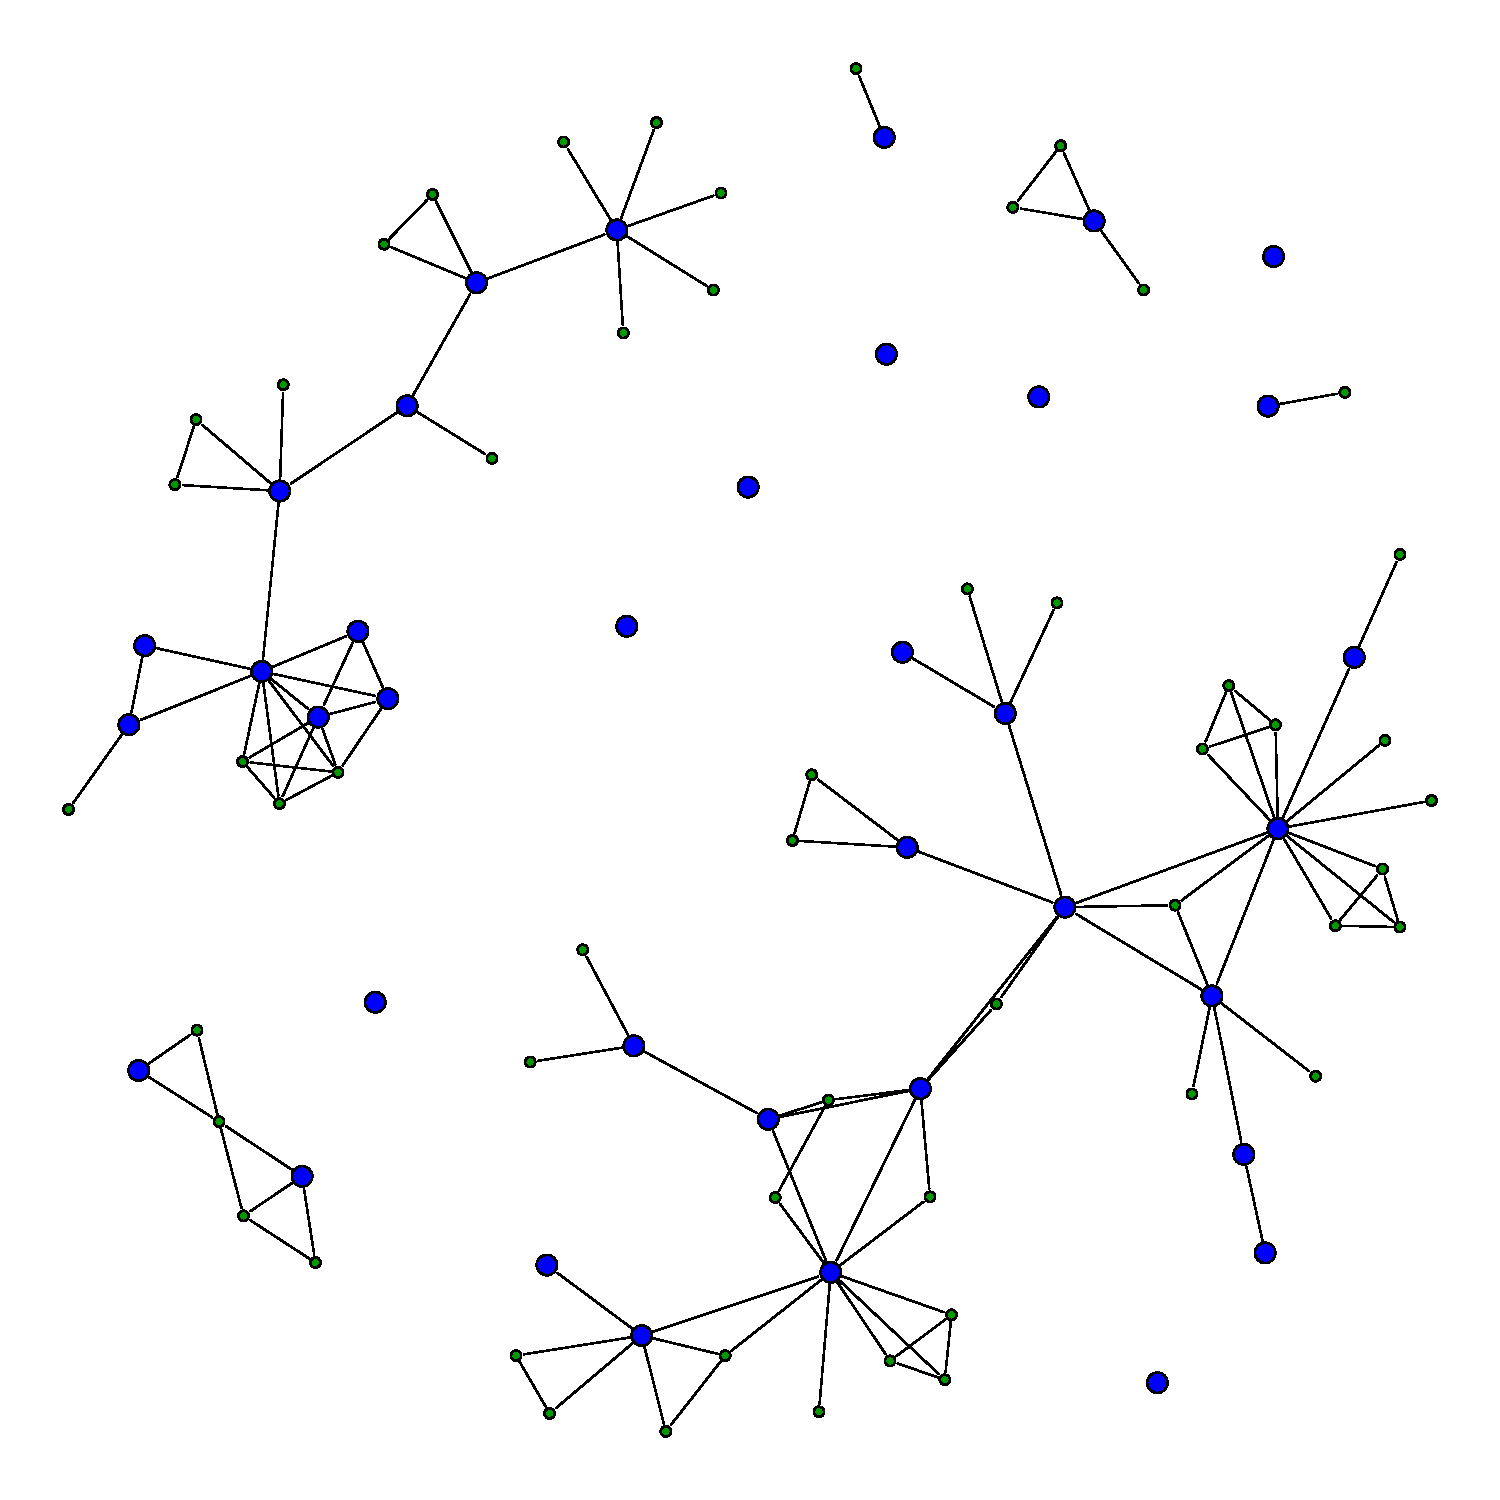
\includegraphics[width=.7\textwidth]{exemplo-grafo}
    \caption{Uma figura simples.\label{fig:subfigures:a}}
  \end{subfigure}
  % ATENÇÃO: Se você deixar uma linha em branco entre as subfiguras,
  % LaTeX vai considerar que cada uma delas pertence a um "parágrafo"
  % diferente e, portanto, vai colocá-las em linhas separadas ao invés
  % de lado a lado.
  \begin{subfigure}{0.4\textwidth}
    \centering
    \begin{turn}{90}
      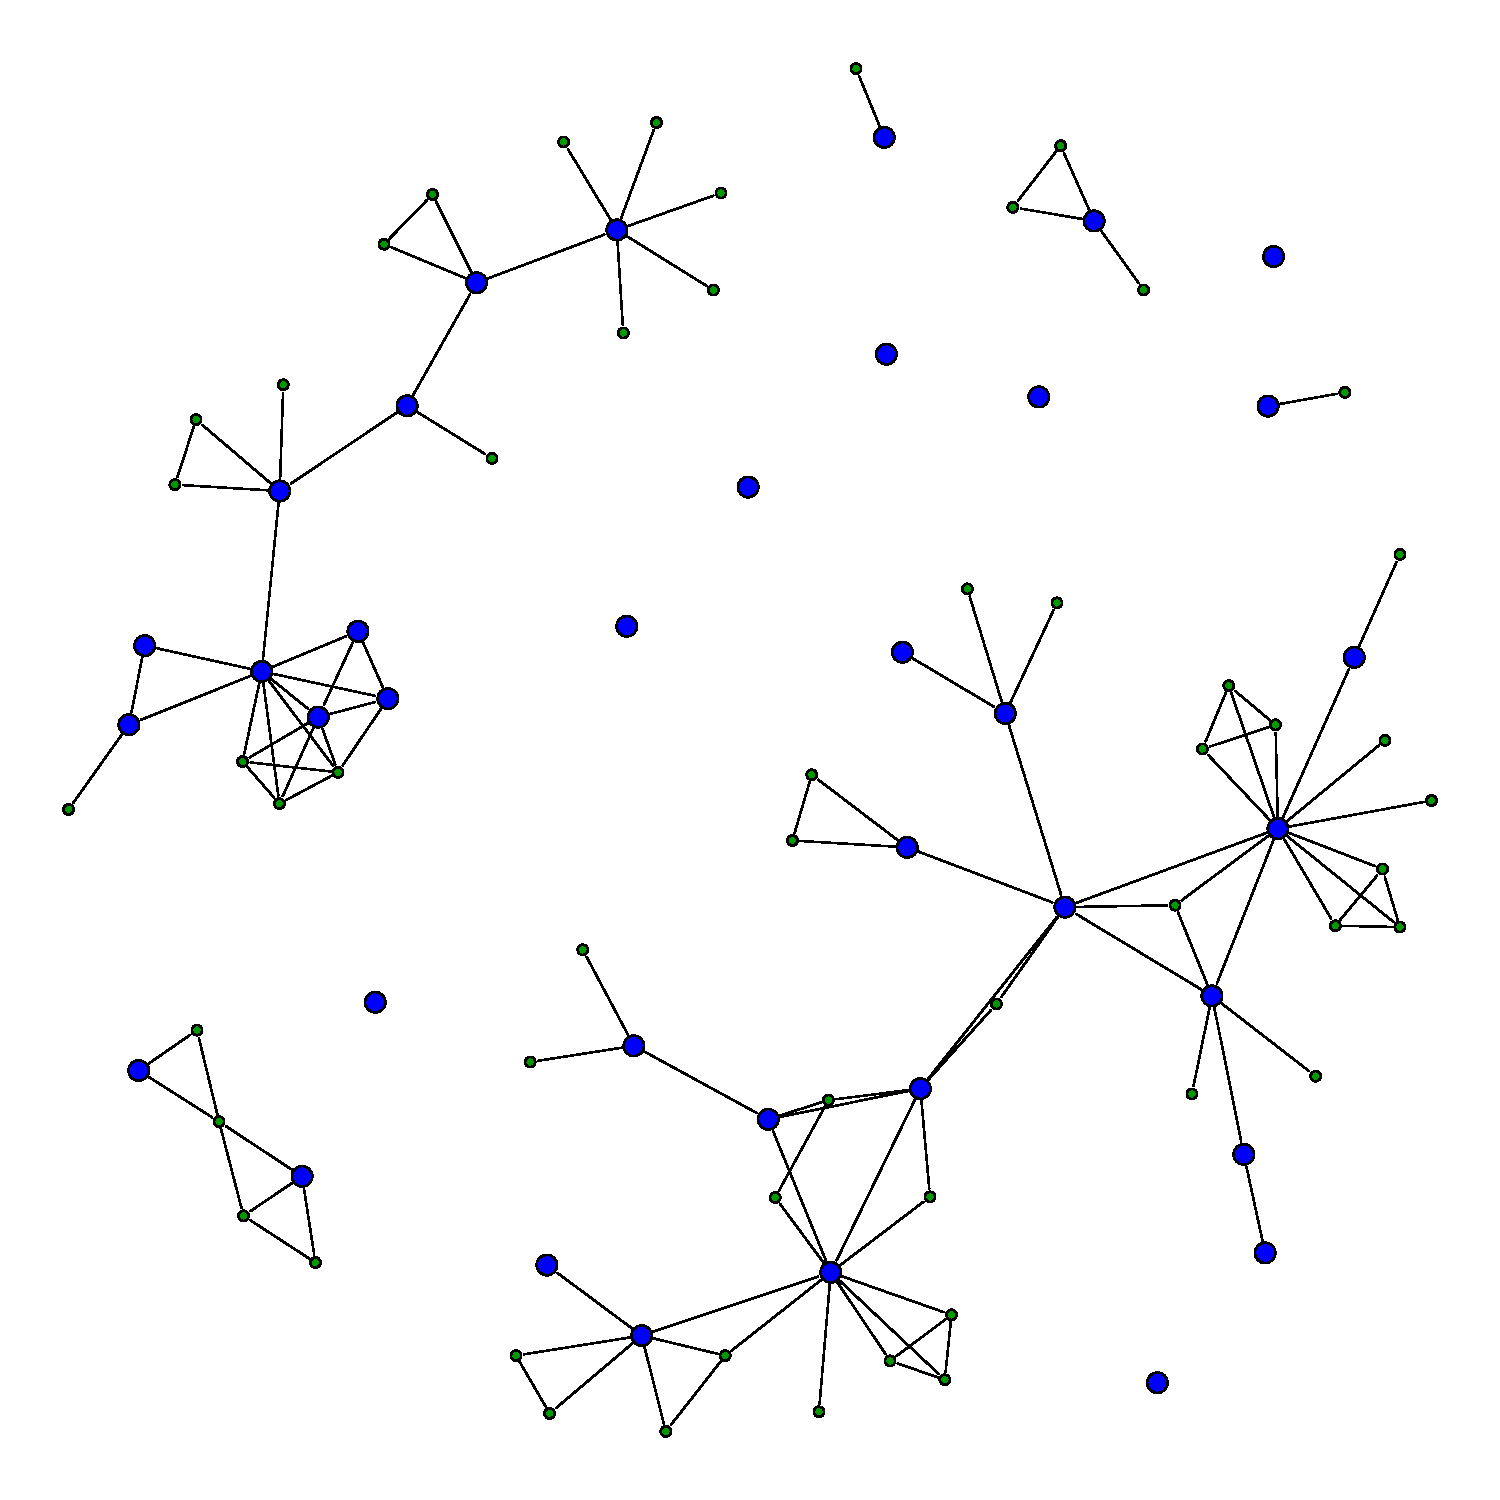
\includegraphics[width=.7\textwidth]{exemplo-grafo}
    \end{turn}
    \caption{O mesmo exemplo, girado.\label{fig:subfigures:b}}
  \end{subfigure}

  \caption{Exemplo de subfiguras.\label{fig:subfigures}}
\end{figure}

Uma ``figura'', na verdade, pode ser qualquer tipo de conteúdo ilustrativo
(um exemplo interessante é o cronograma mostrado na Figura~\ref{fig:gantt}) mas, com a
\textit{package} \textsf{float}, também é possível definir ambientes
específicos para cada tipo de conteúdo adicional (cada um com numeração
independente), como é o caso do Programa~\ref{prog:java}\index{Floats}. Há
mais informações e dicas sobre recursos específicos para inclusão de
código-fonte e pseudocódigo no Apêndice \ref{ap:pseudocode}\footnote{
Observe que o nome do Apêndice (``\ref{ap:pseudocode}'') foi impresso em
uma linha separada, o que não é muito bom visualmente. Para evitar que isso
aconteça (não só no final do parágrafo, mas em qualquer quebra de linha),
faça o que já foi discutido na Seção~\ref{orphanchar} sobre símbolos
matemáticos: utilize um espaço não-separável para fazer referências a
figuras, tabelas, seções etc.: ``\textsf{\dots no
Apêndice\textasciitilde\textbackslash{}ref\{ap:pseudocode\}}''.}.

%%%%%%% Cronograma %%%%%%%

\begin{figure}
  \centering

  \begin{ganttchart}{2017-11}{2018-5}
    \gantttitlecalendar{year,month=shortname} \ganttnewline

    \ganttgroup[progress=45]{Experimento}{2017-11}{2018-2} \ganttnewline
    \ganttbar[progress=100]{
      Preparação\ganttalignnewline
      (compra de insumos)
      }{2017-11}{2017-12} \ganttnewline
    \ganttbar[progress=30]{Execução}{2017-12}{2018-1} \ganttnewline
    \ganttbar[progress=0]{Análise}{2017-12}{2018-2} \ganttnewline

    \ganttgroup[progress=0]{Artigo}{2018-1}{2018-4} \ganttnewline
    \ganttbar[progress=0]{Escrita}{2018-1}{2018-3} \ganttnewline
    \ganttbar[progress=0]{Revisão}{2018-3}{2018-4} \ganttnewline

    \ganttmilestone{Submissão}{2018-4}
  \end{ganttchart}

  \caption{Exemplo de cronograma.\label{fig:gantt}}
\end{figure}

%%%%%%%% Código fonte %%%%%%%%

% Foi utilizado o pacote listings para formatar o código fonte.
% Veja os parâmetros de configuração no arquivo source-code.tex.
\begin{program}
  \index{Java}
  \centering

\begin{lstlisting}[language=Java, style=wider]
  for (i = 0; i < 20; i++)
  {
      // Comentário
      System.out.println("Mensagem...");
  }
\end{lstlisting}

  \caption{Exemplo de laço em Java.\label{prog:java}}
\end{program}

%%%%%

\LaTeX{} pode importar gráficos gerados por \texttt{matplotlib} e por
\texttt{gnuplot} como qualquer outra imagem, mas nesse caso a fonte
usada nesses gráficos provavelmente será diferente do corpo do texto.
Conforme mencionado na Seção~\ref{sec:graficos}, há mecanismos para
resolver esse problema\footnote{Você pode se interessar também pela
package \texttt{gnuplottex}.}, como pode ser visto na
Figura~\ref{fig:graficos}.

\begin{figure}
  \centering
  \begin{subfigure}{.65\textwidth}
    \input{figuras/gnuplot.tkz}
    \caption{\texttt{gnuplot}.\label{fig:gnuplot}}
  \end{subfigure}
  \begin{subfigure}{.3\textwidth}
    %% Creator: Matplotlib, PGF backend
%%
%% To include the figure in your LaTeX document, write
%%   \input{<filename>.pgf}
%%
%% Make sure the required packages are loaded in your preamble
%%   \usepackage{pgf}
%%
%% Figures using additional raster images can only be included by \input if
%% they are in the same directory as the main LaTeX file. For loading figures
%% from other directories you can use the `import` package
%%   \usepackage{import}
%% and then include the figures with
%%   \import{<path to file>}{<filename>.pgf}
%%
%% Matplotlib used the following preamble
%%   \usepackage{fontspec}
%%   \setmainfont{DejaVuSerif.ttf}[Path=/usr/share/matplotlib/mpl-data/fonts/ttf/]
%%   \setsansfont{DejaVuSans.ttf}[Path=/usr/share/matplotlib/mpl-data/fonts/ttf/]
%%   \setmonofont{DejaVuSansMono.ttf}[Path=/usr/share/matplotlib/mpl-data/fonts/ttf/]
%%
\begingroup%
\makeatletter%
\begin{pgfpicture}%
\pgfpathrectangle{\pgfpointorigin}{\pgfqpoint{1.500000in}{2.500000in}}%
\pgfusepath{use as bounding box, clip}%
\begin{pgfscope}%
\pgfsetbuttcap%
\pgfsetmiterjoin%
\definecolor{currentfill}{rgb}{1.000000,1.000000,1.000000}%
\pgfsetfillcolor{currentfill}%
\pgfsetlinewidth{0.000000pt}%
\definecolor{currentstroke}{rgb}{1.000000,1.000000,1.000000}%
\pgfsetstrokecolor{currentstroke}%
\pgfsetdash{}{0pt}%
\pgfpathmoveto{\pgfqpoint{0.000000in}{0.000000in}}%
\pgfpathlineto{\pgfqpoint{1.500000in}{0.000000in}}%
\pgfpathlineto{\pgfqpoint{1.500000in}{2.500000in}}%
\pgfpathlineto{\pgfqpoint{0.000000in}{2.500000in}}%
\pgfpathclose%
\pgfusepath{fill}%
\end{pgfscope}%
\begin{pgfscope}%
\pgfsetbuttcap%
\pgfsetmiterjoin%
\definecolor{currentfill}{rgb}{1.000000,1.000000,1.000000}%
\pgfsetfillcolor{currentfill}%
\pgfsetlinewidth{0.000000pt}%
\definecolor{currentstroke}{rgb}{0.000000,0.000000,0.000000}%
\pgfsetstrokecolor{currentstroke}%
\pgfsetstrokeopacity{0.000000}%
\pgfsetdash{}{0pt}%
\pgfpathmoveto{\pgfqpoint{0.385278in}{0.425278in}}%
\pgfpathlineto{\pgfqpoint{1.452500in}{0.425278in}}%
\pgfpathlineto{\pgfqpoint{1.452500in}{2.452500in}}%
\pgfpathlineto{\pgfqpoint{0.385278in}{2.452500in}}%
\pgfpathclose%
\pgfusepath{fill}%
\end{pgfscope}%
\begin{pgfscope}%
\pgfpathrectangle{\pgfqpoint{0.385278in}{0.425278in}}{\pgfqpoint{1.067222in}{2.027222in}}%
\pgfusepath{clip}%
\pgfsetbuttcap%
\pgfsetmiterjoin%
\definecolor{currentfill}{rgb}{0.121569,0.466667,0.705882}%
\pgfsetfillcolor{currentfill}%
\pgfsetlinewidth{0.000000pt}%
\definecolor{currentstroke}{rgb}{0.000000,0.000000,0.000000}%
\pgfsetstrokecolor{currentstroke}%
\pgfsetstrokeopacity{0.000000}%
\pgfsetdash{}{0pt}%
\pgfpathmoveto{\pgfqpoint{0.433788in}{0.425278in}}%
\pgfpathlineto{\pgfqpoint{0.710988in}{0.425278in}}%
\pgfpathlineto{\pgfqpoint{0.710988in}{1.068840in}}%
\pgfpathlineto{\pgfqpoint{0.433788in}{1.068840in}}%
\pgfpathclose%
\pgfusepath{fill}%
\end{pgfscope}%
\begin{pgfscope}%
\pgfpathrectangle{\pgfqpoint{0.385278in}{0.425278in}}{\pgfqpoint{1.067222in}{2.027222in}}%
\pgfusepath{clip}%
\pgfsetbuttcap%
\pgfsetmiterjoin%
\definecolor{currentfill}{rgb}{0.121569,0.466667,0.705882}%
\pgfsetfillcolor{currentfill}%
\pgfsetlinewidth{0.000000pt}%
\definecolor{currentstroke}{rgb}{0.000000,0.000000,0.000000}%
\pgfsetstrokecolor{currentstroke}%
\pgfsetstrokeopacity{0.000000}%
\pgfsetdash{}{0pt}%
\pgfpathmoveto{\pgfqpoint{0.780289in}{0.425278in}}%
\pgfpathlineto{\pgfqpoint{1.057489in}{0.425278in}}%
\pgfpathlineto{\pgfqpoint{1.057489in}{2.355966in}}%
\pgfpathlineto{\pgfqpoint{0.780289in}{2.355966in}}%
\pgfpathclose%
\pgfusepath{fill}%
\end{pgfscope}%
\begin{pgfscope}%
\pgfpathrectangle{\pgfqpoint{0.385278in}{0.425278in}}{\pgfqpoint{1.067222in}{2.027222in}}%
\pgfusepath{clip}%
\pgfsetbuttcap%
\pgfsetmiterjoin%
\definecolor{currentfill}{rgb}{0.121569,0.466667,0.705882}%
\pgfsetfillcolor{currentfill}%
\pgfsetlinewidth{0.000000pt}%
\definecolor{currentstroke}{rgb}{0.000000,0.000000,0.000000}%
\pgfsetstrokecolor{currentstroke}%
\pgfsetstrokeopacity{0.000000}%
\pgfsetdash{}{0pt}%
\pgfpathmoveto{\pgfqpoint{1.126789in}{0.425278in}}%
\pgfpathlineto{\pgfqpoint{1.403990in}{0.425278in}}%
\pgfpathlineto{\pgfqpoint{1.403990in}{1.712403in}}%
\pgfpathlineto{\pgfqpoint{1.126789in}{1.712403in}}%
\pgfpathclose%
\pgfusepath{fill}%
\end{pgfscope}%
\begin{pgfscope}%
\pgfsetbuttcap%
\pgfsetroundjoin%
\definecolor{currentfill}{rgb}{0.000000,0.000000,0.000000}%
\pgfsetfillcolor{currentfill}%
\pgfsetlinewidth{0.803000pt}%
\definecolor{currentstroke}{rgb}{0.000000,0.000000,0.000000}%
\pgfsetstrokecolor{currentstroke}%
\pgfsetdash{}{0pt}%
\pgfsys@defobject{currentmarker}{\pgfqpoint{0.000000in}{-0.048611in}}{\pgfqpoint{0.000000in}{0.000000in}}{%
\pgfpathmoveto{\pgfqpoint{0.000000in}{0.000000in}}%
\pgfpathlineto{\pgfqpoint{0.000000in}{-0.048611in}}%
\pgfusepath{stroke,fill}%
}%
\begin{pgfscope}%
\pgfsys@transformshift{0.572388in}{0.425278in}%
\pgfsys@useobject{currentmarker}{}%
\end{pgfscope}%
\end{pgfscope}%
\begin{pgfscope}%
\definecolor{textcolor}{rgb}{0.000000,0.000000,0.000000}%
\pgfsetstrokecolor{textcolor}%
\pgfsetfillcolor{textcolor}%
\pgftext[x=0.572388in,y=0.328056in,,top]{\color{textcolor}\rmfamily\fontsize{9.000000}{10.800000}\selectfont SP}%
\end{pgfscope}%
\begin{pgfscope}%
\pgfsetbuttcap%
\pgfsetroundjoin%
\definecolor{currentfill}{rgb}{0.000000,0.000000,0.000000}%
\pgfsetfillcolor{currentfill}%
\pgfsetlinewidth{0.803000pt}%
\definecolor{currentstroke}{rgb}{0.000000,0.000000,0.000000}%
\pgfsetstrokecolor{currentstroke}%
\pgfsetdash{}{0pt}%
\pgfsys@defobject{currentmarker}{\pgfqpoint{0.000000in}{-0.048611in}}{\pgfqpoint{0.000000in}{0.000000in}}{%
\pgfpathmoveto{\pgfqpoint{0.000000in}{0.000000in}}%
\pgfpathlineto{\pgfqpoint{0.000000in}{-0.048611in}}%
\pgfusepath{stroke,fill}%
}%
\begin{pgfscope}%
\pgfsys@transformshift{0.918889in}{0.425278in}%
\pgfsys@useobject{currentmarker}{}%
\end{pgfscope}%
\end{pgfscope}%
\begin{pgfscope}%
\definecolor{textcolor}{rgb}{0.000000,0.000000,0.000000}%
\pgfsetstrokecolor{textcolor}%
\pgfsetfillcolor{textcolor}%
\pgftext[x=0.918889in,y=0.328056in,,top]{\color{textcolor}\rmfamily\fontsize{9.000000}{10.800000}\selectfont RJ}%
\end{pgfscope}%
\begin{pgfscope}%
\pgfsetbuttcap%
\pgfsetroundjoin%
\definecolor{currentfill}{rgb}{0.000000,0.000000,0.000000}%
\pgfsetfillcolor{currentfill}%
\pgfsetlinewidth{0.803000pt}%
\definecolor{currentstroke}{rgb}{0.000000,0.000000,0.000000}%
\pgfsetstrokecolor{currentstroke}%
\pgfsetdash{}{0pt}%
\pgfsys@defobject{currentmarker}{\pgfqpoint{0.000000in}{-0.048611in}}{\pgfqpoint{0.000000in}{0.000000in}}{%
\pgfpathmoveto{\pgfqpoint{0.000000in}{0.000000in}}%
\pgfpathlineto{\pgfqpoint{0.000000in}{-0.048611in}}%
\pgfusepath{stroke,fill}%
}%
\begin{pgfscope}%
\pgfsys@transformshift{1.265390in}{0.425278in}%
\pgfsys@useobject{currentmarker}{}%
\end{pgfscope}%
\end{pgfscope}%
\begin{pgfscope}%
\definecolor{textcolor}{rgb}{0.000000,0.000000,0.000000}%
\pgfsetstrokecolor{textcolor}%
\pgfsetfillcolor{textcolor}%
\pgftext[x=1.265390in,y=0.328056in,,top]{\color{textcolor}\rmfamily\fontsize{9.000000}{10.800000}\selectfont MG}%
\end{pgfscope}%
\begin{pgfscope}%
\definecolor{textcolor}{rgb}{0.000000,0.000000,0.000000}%
\pgfsetstrokecolor{textcolor}%
\pgfsetfillcolor{textcolor}%
\pgftext[x=0.918889in,y=0.151528in,,top]{\color{textcolor}\rmfamily\fontsize{9.000000}{10.800000}\selectfont \textit{Estado}}%
\end{pgfscope}%
\begin{pgfscope}%
\pgfsetbuttcap%
\pgfsetroundjoin%
\definecolor{currentfill}{rgb}{0.000000,0.000000,0.000000}%
\pgfsetfillcolor{currentfill}%
\pgfsetlinewidth{0.803000pt}%
\definecolor{currentstroke}{rgb}{0.000000,0.000000,0.000000}%
\pgfsetstrokecolor{currentstroke}%
\pgfsetdash{}{0pt}%
\pgfsys@defobject{currentmarker}{\pgfqpoint{-0.048611in}{0.000000in}}{\pgfqpoint{0.000000in}{0.000000in}}{%
\pgfpathmoveto{\pgfqpoint{0.000000in}{0.000000in}}%
\pgfpathlineto{\pgfqpoint{-0.048611in}{0.000000in}}%
\pgfusepath{stroke,fill}%
}%
\begin{pgfscope}%
\pgfsys@transformshift{0.385278in}{0.425278in}%
\pgfsys@useobject{currentmarker}{}%
\end{pgfscope}%
\end{pgfscope}%
\begin{pgfscope}%
\definecolor{textcolor}{rgb}{0.000000,0.000000,0.000000}%
\pgfsetstrokecolor{textcolor}%
\pgfsetfillcolor{textcolor}%
\pgftext[x=0.208527in,y=0.377792in,left,base]{\color{textcolor}\rmfamily\fontsize{9.000000}{10.800000}\selectfont 0}%
\end{pgfscope}%
\begin{pgfscope}%
\pgfsetbuttcap%
\pgfsetroundjoin%
\definecolor{currentfill}{rgb}{0.000000,0.000000,0.000000}%
\pgfsetfillcolor{currentfill}%
\pgfsetlinewidth{0.803000pt}%
\definecolor{currentstroke}{rgb}{0.000000,0.000000,0.000000}%
\pgfsetstrokecolor{currentstroke}%
\pgfsetdash{}{0pt}%
\pgfsys@defobject{currentmarker}{\pgfqpoint{-0.048611in}{0.000000in}}{\pgfqpoint{0.000000in}{0.000000in}}{%
\pgfpathmoveto{\pgfqpoint{0.000000in}{0.000000in}}%
\pgfpathlineto{\pgfqpoint{-0.048611in}{0.000000in}}%
\pgfusepath{stroke,fill}%
}%
\begin{pgfscope}%
\pgfsys@transformshift{0.385278in}{0.747059in}%
\pgfsys@useobject{currentmarker}{}%
\end{pgfscope}%
\end{pgfscope}%
\begin{pgfscope}%
\definecolor{textcolor}{rgb}{0.000000,0.000000,0.000000}%
\pgfsetstrokecolor{textcolor}%
\pgfsetfillcolor{textcolor}%
\pgftext[x=0.208527in,y=0.699574in,left,base]{\color{textcolor}\rmfamily\fontsize{9.000000}{10.800000}\selectfont 1}%
\end{pgfscope}%
\begin{pgfscope}%
\pgfsetbuttcap%
\pgfsetroundjoin%
\definecolor{currentfill}{rgb}{0.000000,0.000000,0.000000}%
\pgfsetfillcolor{currentfill}%
\pgfsetlinewidth{0.803000pt}%
\definecolor{currentstroke}{rgb}{0.000000,0.000000,0.000000}%
\pgfsetstrokecolor{currentstroke}%
\pgfsetdash{}{0pt}%
\pgfsys@defobject{currentmarker}{\pgfqpoint{-0.048611in}{0.000000in}}{\pgfqpoint{0.000000in}{0.000000in}}{%
\pgfpathmoveto{\pgfqpoint{0.000000in}{0.000000in}}%
\pgfpathlineto{\pgfqpoint{-0.048611in}{0.000000in}}%
\pgfusepath{stroke,fill}%
}%
\begin{pgfscope}%
\pgfsys@transformshift{0.385278in}{1.068840in}%
\pgfsys@useobject{currentmarker}{}%
\end{pgfscope}%
\end{pgfscope}%
\begin{pgfscope}%
\definecolor{textcolor}{rgb}{0.000000,0.000000,0.000000}%
\pgfsetstrokecolor{textcolor}%
\pgfsetfillcolor{textcolor}%
\pgftext[x=0.208527in,y=1.021355in,left,base]{\color{textcolor}\rmfamily\fontsize{9.000000}{10.800000}\selectfont 2}%
\end{pgfscope}%
\begin{pgfscope}%
\pgfsetbuttcap%
\pgfsetroundjoin%
\definecolor{currentfill}{rgb}{0.000000,0.000000,0.000000}%
\pgfsetfillcolor{currentfill}%
\pgfsetlinewidth{0.803000pt}%
\definecolor{currentstroke}{rgb}{0.000000,0.000000,0.000000}%
\pgfsetstrokecolor{currentstroke}%
\pgfsetdash{}{0pt}%
\pgfsys@defobject{currentmarker}{\pgfqpoint{-0.048611in}{0.000000in}}{\pgfqpoint{0.000000in}{0.000000in}}{%
\pgfpathmoveto{\pgfqpoint{0.000000in}{0.000000in}}%
\pgfpathlineto{\pgfqpoint{-0.048611in}{0.000000in}}%
\pgfusepath{stroke,fill}%
}%
\begin{pgfscope}%
\pgfsys@transformshift{0.385278in}{1.390622in}%
\pgfsys@useobject{currentmarker}{}%
\end{pgfscope}%
\end{pgfscope}%
\begin{pgfscope}%
\definecolor{textcolor}{rgb}{0.000000,0.000000,0.000000}%
\pgfsetstrokecolor{textcolor}%
\pgfsetfillcolor{textcolor}%
\pgftext[x=0.208527in,y=1.343136in,left,base]{\color{textcolor}\rmfamily\fontsize{9.000000}{10.800000}\selectfont 3}%
\end{pgfscope}%
\begin{pgfscope}%
\pgfsetbuttcap%
\pgfsetroundjoin%
\definecolor{currentfill}{rgb}{0.000000,0.000000,0.000000}%
\pgfsetfillcolor{currentfill}%
\pgfsetlinewidth{0.803000pt}%
\definecolor{currentstroke}{rgb}{0.000000,0.000000,0.000000}%
\pgfsetstrokecolor{currentstroke}%
\pgfsetdash{}{0pt}%
\pgfsys@defobject{currentmarker}{\pgfqpoint{-0.048611in}{0.000000in}}{\pgfqpoint{0.000000in}{0.000000in}}{%
\pgfpathmoveto{\pgfqpoint{0.000000in}{0.000000in}}%
\pgfpathlineto{\pgfqpoint{-0.048611in}{0.000000in}}%
\pgfusepath{stroke,fill}%
}%
\begin{pgfscope}%
\pgfsys@transformshift{0.385278in}{1.712403in}%
\pgfsys@useobject{currentmarker}{}%
\end{pgfscope}%
\end{pgfscope}%
\begin{pgfscope}%
\definecolor{textcolor}{rgb}{0.000000,0.000000,0.000000}%
\pgfsetstrokecolor{textcolor}%
\pgfsetfillcolor{textcolor}%
\pgftext[x=0.208527in,y=1.664918in,left,base]{\color{textcolor}\rmfamily\fontsize{9.000000}{10.800000}\selectfont 4}%
\end{pgfscope}%
\begin{pgfscope}%
\pgfsetbuttcap%
\pgfsetroundjoin%
\definecolor{currentfill}{rgb}{0.000000,0.000000,0.000000}%
\pgfsetfillcolor{currentfill}%
\pgfsetlinewidth{0.803000pt}%
\definecolor{currentstroke}{rgb}{0.000000,0.000000,0.000000}%
\pgfsetstrokecolor{currentstroke}%
\pgfsetdash{}{0pt}%
\pgfsys@defobject{currentmarker}{\pgfqpoint{-0.048611in}{0.000000in}}{\pgfqpoint{0.000000in}{0.000000in}}{%
\pgfpathmoveto{\pgfqpoint{0.000000in}{0.000000in}}%
\pgfpathlineto{\pgfqpoint{-0.048611in}{0.000000in}}%
\pgfusepath{stroke,fill}%
}%
\begin{pgfscope}%
\pgfsys@transformshift{0.385278in}{2.034184in}%
\pgfsys@useobject{currentmarker}{}%
\end{pgfscope}%
\end{pgfscope}%
\begin{pgfscope}%
\definecolor{textcolor}{rgb}{0.000000,0.000000,0.000000}%
\pgfsetstrokecolor{textcolor}%
\pgfsetfillcolor{textcolor}%
\pgftext[x=0.208527in,y=1.986699in,left,base]{\color{textcolor}\rmfamily\fontsize{9.000000}{10.800000}\selectfont 5}%
\end{pgfscope}%
\begin{pgfscope}%
\pgfsetbuttcap%
\pgfsetroundjoin%
\definecolor{currentfill}{rgb}{0.000000,0.000000,0.000000}%
\pgfsetfillcolor{currentfill}%
\pgfsetlinewidth{0.803000pt}%
\definecolor{currentstroke}{rgb}{0.000000,0.000000,0.000000}%
\pgfsetstrokecolor{currentstroke}%
\pgfsetdash{}{0pt}%
\pgfsys@defobject{currentmarker}{\pgfqpoint{-0.048611in}{0.000000in}}{\pgfqpoint{0.000000in}{0.000000in}}{%
\pgfpathmoveto{\pgfqpoint{0.000000in}{0.000000in}}%
\pgfpathlineto{\pgfqpoint{-0.048611in}{0.000000in}}%
\pgfusepath{stroke,fill}%
}%
\begin{pgfscope}%
\pgfsys@transformshift{0.385278in}{2.355966in}%
\pgfsys@useobject{currentmarker}{}%
\end{pgfscope}%
\end{pgfscope}%
\begin{pgfscope}%
\definecolor{textcolor}{rgb}{0.000000,0.000000,0.000000}%
\pgfsetstrokecolor{textcolor}%
\pgfsetfillcolor{textcolor}%
\pgftext[x=0.208527in,y=2.308480in,left,base]{\color{textcolor}\rmfamily\fontsize{9.000000}{10.800000}\selectfont 6}%
\end{pgfscope}%
\begin{pgfscope}%
\definecolor{textcolor}{rgb}{0.000000,0.000000,0.000000}%
\pgfsetstrokecolor{textcolor}%
\pgfsetfillcolor{textcolor}%
\pgftext[x=0.152971in,y=1.438889in,,bottom,rotate=90.000000]{\color{textcolor}\rmfamily\fontsize{9.000000}{10.800000}\selectfont \(\displaystyle \mu\)}%
\end{pgfscope}%
\begin{pgfscope}%
\pgfsetrectcap%
\pgfsetmiterjoin%
\pgfsetlinewidth{0.803000pt}%
\definecolor{currentstroke}{rgb}{0.000000,0.000000,0.000000}%
\pgfsetstrokecolor{currentstroke}%
\pgfsetdash{}{0pt}%
\pgfpathmoveto{\pgfqpoint{0.385278in}{0.425278in}}%
\pgfpathlineto{\pgfqpoint{0.385278in}{2.452500in}}%
\pgfusepath{stroke}%
\end{pgfscope}%
\begin{pgfscope}%
\pgfsetrectcap%
\pgfsetmiterjoin%
\pgfsetlinewidth{0.803000pt}%
\definecolor{currentstroke}{rgb}{0.000000,0.000000,0.000000}%
\pgfsetstrokecolor{currentstroke}%
\pgfsetdash{}{0pt}%
\pgfpathmoveto{\pgfqpoint{1.452500in}{0.425278in}}%
\pgfpathlineto{\pgfqpoint{1.452500in}{2.452500in}}%
\pgfusepath{stroke}%
\end{pgfscope}%
\begin{pgfscope}%
\pgfsetrectcap%
\pgfsetmiterjoin%
\pgfsetlinewidth{0.803000pt}%
\definecolor{currentstroke}{rgb}{0.000000,0.000000,0.000000}%
\pgfsetstrokecolor{currentstroke}%
\pgfsetdash{}{0pt}%
\pgfpathmoveto{\pgfqpoint{0.385278in}{0.425278in}}%
\pgfpathlineto{\pgfqpoint{1.452500in}{0.425278in}}%
\pgfusepath{stroke}%
\end{pgfscope}%
\begin{pgfscope}%
\pgfsetrectcap%
\pgfsetmiterjoin%
\pgfsetlinewidth{0.803000pt}%
\definecolor{currentstroke}{rgb}{0.000000,0.000000,0.000000}%
\pgfsetstrokecolor{currentstroke}%
\pgfsetdash{}{0pt}%
\pgfpathmoveto{\pgfqpoint{0.385278in}{2.452500in}}%
\pgfpathlineto{\pgfqpoint{1.452500in}{2.452500in}}%
\pgfusepath{stroke}%
\end{pgfscope}%
\end{pgfpicture}%
\makeatother%
\endgroup%

    \caption{\texttt{matplotlib}.\label{fig:matplotlib}}
  \end{subfigure}
	\caption{Exemplos de gráficos gerados externamente}\label{fig:graficos}
\end{figure}

Finalmente, talvez você precise organizar a apresentação da informação na forma de
tabelas\index{Floats}\footnote{Para defini-las com \LaTeX{}, pode valer a pena usar o
sítio \url{www.tablesgenerator.com}.}; Um exemplo simples é a Tabela~\ref{tab:amino_acidos}.

%%%%%%%% Tabelas lado-a-lado %%%%%%%%

\begin{table}
\centering

  \hspace*{\fill}
  \begin{subtable}[b]{0.42\textwidth}
    % \rowcolors é definida pela package xcolor;
    % veja também os recursos da package colortbl
    \rowcolors{2}{lightgray!70}{white}
    \centering
    \begin{tabular}{ccl}
      \toprule
      Código      & Abreviatura  & \makecell{Nome\\completo} \\
      \midrule
      \texttt{A}  & Ala          & Alanina \\
      \texttt{C}  & Cys          & Cisteína \\
      ...         & ...          & ... \\
      \texttt{W}  & Trp          & Triptofano \\
      \texttt{Y}  & Tyr          & Tirosina \\
      \bottomrule
    \end{tabular}
    \caption{Com linhas de cores alternadas.}
  \end{subtable}
  % Como mencionado mais acima, não deixe linhas em branco aqui
  \hspace*{\fill}\hspace*{\fill}\hspace*{\fill}
  \begin{subtable}[b]{0.37\textwidth}
    \centering
    \begin{tabular}{ccl}
      \rothead{Código} & \rothead{Abreviatura} & \rothead{Nome\\completo} \\
      \midrule
      \texttt{A}       & Ala                   & Alanina \\
      \texttt{C}       & Cys                   & Cisteína \\
      ...              & ...                   & ... \\
      \texttt{W}       & Trp                   & Triptofano \\
      \texttt{Y}       & Tyr                   & Tirosina \\
      \bottomrule
    \end{tabular}
    \caption{Com cabeçalhos girados.}
  \end{subtable}
  \hspace*{\fill}

  \caption{Exemplos de tabelas (códigos, abreviaturas e nomes dos aminoácidos).\label{tab:amino_acidos}}
\end{table}

Se a tabela tem muitas linhas e, portanto, não cabe em uma única página, é
possível fazê-la continuar ao longo de várias páginas com a \textit{package}
\textsf{longtable}, como é o caso da Tabela~\ref{tab:numeros}. Nesse caso,
a tabela não é um \textit{float} e, portanto, ela aparece de acordo com a
sequência normal do texto. Se, além de muito longa, a tabela for também
muito larga, você pode usar o comando \textsf{landscape} (da
\textit{package} \textsf{pdflscape}) em conjunto com \textsf{longtable}
para imprimi-la em modo paisagem ao longo de várias páginas. A
Tabela~\ref{tab:numeros} tem essa configuração comentada; experimente
des-comentar as linhas correspondentes\footnote{Observe que, nesse caso,
vai sempre haver uma quebra de página no texto para fazer a tabela
começar em uma página em modo paisagem.}.

%%%%%%%% Tabela longa em várias páginas %%%%%%%%

%%%% É possível fazer esta mesma tabela em modo paisagem des-comentando
%%%% esta linha e a correspondente no final da tabela
%\begin{landscape}
\begin{longtable}[c]{|c|c|c|c|c|c|c|c|c|c|c|c|c|}

%%%%%%%%%%%%
% O cabeçalho da tabela na primeira página em que ela aparece.

\hline
% Como a tabela pode se estender por várias páginas, precisamos tomar
% cuidado especial com \caption e \label: se esses comandos forem
% executados mais de uma vez, a lista de tabelas e as referências à
% tabela ficarão incorretas. Há diversas soluções, mas a mais simples
% é usar "\caption[]", que não coloca a tabela na lista de tabelas, e
% incluí-la manualmente na lista apenas uma vez aqui junto com o \label.
\captionlistentry{Exemplo de tabela com valores numéricos.}\label{tab:numeros}

\emph{Lim.} &
\multicolumn{3}{c|}{MGWT} &
\multicolumn{3}{c|}{AMI} &
\multicolumn{3}{c|}{\emph{Spectrum} de Fourier} &
\multicolumn{3}{c|}{Caract. espectrais} \\

\cline{2-4} \cline{5-7} \cline{8-10} \cline{11-13} &
\emph{Sn} & \emph{Sp} & \emph{AC} &
\emph{Sn} & \emph{Sp} & \emph{AC} &
\emph{Sn} & \emph{Sp} & \emph{AC} &
\emph{Sn} & \emph{Sp} & \emph{AC} \\

\hline \hline

\endfirsthead % Final do cabeçalho que aparece na primeira página

%%%%%%%%%%%%
% O cabeçalho da tabela em todas as páginas em que ela aparece
% exceto a primeira; aqui, igual ao anterior

\hline

\emph{Lim.} &
\multicolumn{3}{c|}{MGWT} &
\multicolumn{3}{c|}{AMI} &
\multicolumn{3}{c|}{\emph{Spectrum} de Fourier} &
\multicolumn{3}{c|}{Caract. espectrais} \\

\cline{2-4} \cline{5-7} \cline{8-10} \cline{11-13} &
\emph{Sn} & \emph{Sp} & \emph{AC} &
\emph{Sn} & \emph{Sp} & \emph{AC} &
\emph{Sn} & \emph{Sp} & \emph{AC} &
\emph{Sn} & \emph{Sp} & \emph{AC} \\

\hline \hline

\endhead % Final do cabeçalho das páginas seguintes à primeira

%%%%%%%%%%%%
% O rodapé da tabela em todas as páginas em que ela aparece
% exceto a última

\hline

\multicolumn{13}{|r|}{\textit{continua}\enspace$\longrightarrow$}\\

\hline

% Como usamos \captionlistentry mais acima, usamos "[]" aqui.
\caption[]{Exemplo de tabela com valores numéricos.}

\endfoot % Final do rodapé que aparece em todas as páginas exceto a última

%%%%%%%%%%%%
% O rodapé da tabela na última página em que ela aparece

\hline

% Como usamos \captionlistentry mais acima, usamos "[]" aqui.
\caption[]{Exemplo de tabela com valores numéricos.}

\endlastfoot % Final do rodapé da última página

%%%%%%%%%%%%
% O conteúdo da tabela de fato.

 1 & 1.00 & 0.16 & 0.08 & 1.00 & 0.16 & 0.08 & 1.00 & 0.16 & 0.08 & 1.00 & 0.16 & 0.08 \\
 2 & 1.00 & 0.16 & 0.09 & 1.00 & 0.16 & 0.09 & 1.00 & 0.16 & 0.09 & 1.00 & 0.16 & 0.09 \\
 3 & 1.00 & 0.16 & 0.10 & 1.00 & 0.16 & 0.10 & 1.00 & 0.16 & 0.10 & 1.00 & 0.16 & 0.10 \\
 4 & 1.00 & 0.16 & 0.10 & 1.00 & 0.16 & 0.10 & 1.00 & 0.16 & 0.10 & 1.00 & 0.16 & 0.10 \\
 5 & 1.00 & 0.16 & 0.11 & 1.00 & 0.16 & 0.11 & 1.00 & 0.16 & 0.11 & 1.00 & 0.16 & 0.11 \\
 6 & 1.00 & 0.16 & 0.12 & 1.00 & 0.16 & 0.12 & 1.00 & 0.16 & 0.12 & 1.00 & 0.16 & 0.12 \\
 7 & 1.00 & 0.17 & 0.12 & 1.00 & 0.17 & 0.12 & 1.00 & 0.17 & 0.12 & 1.00 & 0.17 & 0.13 \\
 8 & 1.00 & 0.17 & 0.13 & 1.00 & 0.17 & 0.13 & 1.00 & 0.17 & 0.13 & 1.00 & 0.17 & 0.13 \\
 9 & 1.00 & 0.17 & 0.14 & 1.00 & 0.17 & 0.14 & 1.00 & 0.17 & 0.14 & 1.00 & 0.17 & 0.14 \\
10 & 1.00 & 0.17 & 0.15 & 1.00 & 0.17 & 0.15 & 1.00 & 0.17 & 0.15 & 1.00 & 0.17 & 0.15 \\
11 & 1.00 & 0.17 & 0.15 & 1.00 & 0.17 & 0.15 & 1.00 & 0.17 & 0.15 & 1.00 & 0.17 & 0.15 \\
12 & 1.00 & 0.18 & 0.16 & 1.00 & 0.18 & 0.16 & 1.00 & 0.18 & 0.16 & 1.00 & 0.18 & 0.16 \\
13 & 1.00 & 0.18 & 0.17 & 1.00 & 0.18 & 0.17 & 1.00 & 0.18 & 0.17 & 1.00 & 0.18 & 0.17 \\
14 & 1.00 & 0.18 & 0.17 & 1.00 & 0.18 & 0.17 & 1.00 & 0.18 & 0.17 & 1.00 & 0.18 & 0.17 \\
% Como nesta página há uma nota de rodapé, a linha separadora da
% nota e o final da tabela ficam muito próximos; vamos forçar uma
% quebra de página uma linha antes para resolver isso.
\pagebreak
15 & 1.00 & 0.18 & 0.18 & 1.00 & 0.18 & 0.18 & 1.00 & 0.18 & 0.18 & 1.00 & 0.18 & 0.18 \\
16 & 1.00 & 0.18 & 0.19 & 1.00 & 0.18 & 0.19 & 1.00 & 0.18 & 0.19 & 1.00 & 0.18 & 0.19 \\
17 & 1.00 & 0.19 & 0.19 & 1.00 & 0.19 & 0.19 & 1.00 & 0.19 & 0.19 & 1.00 & 0.19 & 0.19 \\
18 & 1.00 & 0.19 & 0.20 & 1.00 & 0.19 & 0.20 & 1.00 & 0.19 & 0.20 & 1.00 & 0.19 & 0.20 \\
19 & 1.00 & 0.19 & 0.21 & 1.00 & 0.19 & 0.21 & 1.00 & 0.19 & 0.21 & 1.00 & 0.19 & 0.21 \\
20 & 1.00 & 0.19 & 0.22 & 1.00 & 0.19 & 0.22 & 1.00 & 0.19 & 0.22 & 1.00 & 0.19 & 0.22 \\
21 & 1.00 & 0.19 & 0.22 & 1.00 & 0.19 & 0.22 & 1.00 & 0.19 & 0.22 & 1.00 & 0.19 & 0.22 \\
22 & 1.00 & 0.19 & 0.22 & 1.00 & 0.19 & 0.22 & 1.00 & 0.19 & 0.22 & 1.00 & 0.19 & 0.22 \\
23 & 1.00 & 0.19 & 0.22 & 1.00 & 0.19 & 0.22 & 1.00 & 0.19 & 0.22 & 1.00 & 0.19 & 0.22 \\
24 & 1.00 & 0.19 & 0.22 & 1.00 & 0.19 & 0.22 & 1.00 & 0.19 & 0.22 & 1.00 & 0.19 & 0.22 \\
25 & 1.00 & 0.19 & 0.22 & 1.00 & 0.19 & 0.22 & 1.00 & 0.19 & 0.22 & 1.00 & 0.19 & 0.22 \\
26 & 1.00 & 0.19 & 0.22 & 1.00 & 0.19 & 0.22 & 1.00 & 0.19 & 0.22 & 1.00 & 0.19 & 0.22 \\
27 & 1.00 & 0.19 & 0.22 & 1.00 & 0.19 & 0.22 & 1.00 & 0.19 & 0.22 & 1.00 & 0.19 & 0.22 \\
28 & 1.00 & 0.19 & 0.22 & 1.00 & 0.19 & 0.22 & 1.00 & 0.19 & 0.22 & 1.00 & 0.19 & 0.22 \\
29 & 1.00 & 0.19 & 0.22 & 1.00 & 0.19 & 0.22 & 1.00 & 0.19 & 0.22 & 1.00 & 0.19 & 0.22 \\
30 & 1.00 & 0.19 & 0.22 & 1.00 & 0.19 & 0.22 & 1.00 & 0.19 & 0.22 & 1.00 & 0.19 & 0.22 \\
31 & 1.00 & 0.19 & 0.22 & 1.00 & 0.19 & 0.22 & 1.00 & 0.19 & 0.22 & 1.00 & 0.19 & 0.22 \\
32 & 1.00 & 0.19 & 0.22 & 1.00 & 0.19 & 0.22 & 1.00 & 0.19 & 0.22 & 1.00 & 0.19 & 0.22 \\
33 & 1.00 & 0.19 & 0.22 & 1.00 & 0.19 & 0.22 & 1.00 & 0.19 & 0.22 & 1.00 & 0.19 & 0.22 \\
34 & 1.00 & 0.19 & 0.22 & 1.00 & 0.19 & 0.22 & 1.00 & 0.19 & 0.22 & 1.00 & 0.19 & 0.22 \\
35 & 1.00 & 0.19 & 0.22 & 1.00 & 0.19 & 0.22 & 1.00 & 0.19 & 0.22 & 1.00 & 0.19 & 0.22 \\
36 & 1.00 & 0.19 & 0.22 & 1.00 & 0.19 & 0.22 & 1.00 & 0.19 & 0.22 & 1.00 & 0.19 & 0.22 \\
37 & 1.00 & 0.19 & 0.22 & 1.00 & 0.19 & 0.22 & 1.00 & 0.19 & 0.22 & 1.00 & 0.19 & 0.22 \\
38 & 1.00 & 0.19 & 0.22 & 1.00 & 0.19 & 0.22 & 1.00 & 0.19 & 0.22 & 1.00 & 0.19 & 0.22 \\
39 & 1.00 & 0.19 & 0.22 & 1.00 & 0.19 & 0.22 & 1.00 & 0.19 & 0.22 & 1.00 & 0.19 & 0.22 \\
40 & 1.00 & 0.19 & 0.22 & 1.00 & 0.19 & 0.22 & 1.00 & 0.19 & 0.22 & 1.00 & 0.19 & 0.22 \\
\end{longtable}
%\end{landscape}

Tabelas mais complexas são um tanto trabalhosas em \LaTeX{}; a
Tabela~\ref{tab:ficha} mostra como construir uma tabela em forma de ficha.
Além de complexa, ela é larga e, portanto, deve ser impressa em modo
paisagem. No entanto, usamos um outro mecanismo para girar a tabela: o
comando \textsf{sidewaystable} (da \textit{package} \textsf{rotating}).
Com esse mecanismo, ela continua sendo um \textit{float} (e, portanto,
não força quebras de página no meio do texto), mas sempre é impressa em
uma página separada.

Resumindo:

\begin{itemize}
  \item Se uma tabela cabe em uma página, defina-a como um \textit{float};
  \item se cabe em uma página mas é muito larga e precisa ser impressa em
        modo paisagem, use \textsf{sidewaystable} (que também é um \textit{float});
  \item se não cabe em uma página por ser muito longa, use \textsf{longtable};
  \item se não cabe em uma página por ser muito longa e precisa ser impressa
        em modo paisagem por ser muito larga, use \textsf{longtable} em
        conjunto com \textsf{landscape}.
\end{itemize}

%%%%%%%% Tabela em forma de ficha %%%%%%%%

% Aumenta o espaçamento entre as linhas da tabela (default: 0pt)
\setlength\extrarowheight{4pt}

% sidewaystable e comandos relacionados são definidos na package rotating
\begin{sidewaystable}
\centering

\begin{tabular}{|M{0.265}|M{0.073}|M{0.084}|M{0.073}|M{0.073}|M{0.08}|M{0.082}|M{0.067}|}
  \hline
    \textbf{Experimento número:} & \multicolumn{2}{c|}{1} & \multicolumn{4}{c|}{\textbf{Data:}} & jan 2017
  \tabularnewline \hline
    \textbf{Título:} & \multicolumn{7}{c|}{Medições iniciais}
  \tabularnewline \hline
    \textbf{Tipo de experimento:} & \multicolumn{7}{c|}{Levantamento quantitativo}
  \tabularnewline \hline \hline
    \textbf{Locais}          & São Paulo & Rio de Janeiro & Porto Alegre & Recife & Manaus & Brasília & Rio Branco
  \tabularnewline \thickhline
    \textbf{Valores obtidos} & 0.2       & 0.3            & 0.2          & 0.7    & 0.5    & 0.1      & 0.4
  \tabularnewline \hline
\end{tabular}

\caption{Exemplo de tabela similar a uma ficha.\label{tab:ficha}}
\end{sidewaystable}

% Redefinindo para o valor default
\setlength\extrarowheight{0pt}

\par
